% Options for packages loaded elsewhere
\PassOptionsToPackage{unicode}{hyperref}
\PassOptionsToPackage{hyphens}{url}
\documentclass[
  12pt,
  a4paper
]{article}

% --- 页面布局 ---
\usepackage{geometry}
\geometry{
  left=2.5cm,
  right=2.5cm,
  top=2.5cm,
  bottom=2.5cm
}

% --- 行距 (中文阅读舒适) ---
\usepackage{setspace}
\setstretch{1.35}

\usepackage{xcolor}
\usepackage{amsmath,amssymb}
\setcounter{secnumdepth}{-\maxdimen} % remove section numbering
\usepackage{iftex}
\ifPDFTeX
  \usepackage[T1]{fontenc}
  \usepackage[utf8]{inputenc}
  \usepackage{textcomp} % provide euro and other symbols
  \usepackage{lmodern}
\else % if luatex or xetex
  \usepackage{unicode-math} % this also loads fontspec
  \defaultfontfeatures{Scale=MatchLowercase}
  \defaultfontfeatures[\rmfamily]{Ligatures=TeX,Scale=1}
  % --- 拉丁正文字体: DejaVu Serif (覆盖希腊/数学符号Unicode) ---
  \setmainfont{DejaVu Serif}
  % --- CJK 中文支持 ---
  \usepackage{xeCJK}
  \setCJKmainfont{Noto Serif CJK SC}[
    BoldFont=Noto Sans CJK SC
  ]
  \setCJKsansfont{Noto Sans CJK SC}
  \setCJKmonofont{Noto Sans CJK SC}
  \xeCJKsetup{CJKmath=false}
\fi
% Use upquote if available, for straight quotes in verbatim environments
\IfFileExists{upquote.sty}{\usepackage{upquote}}{}
\IfFileExists{microtype.sty}{% use microtype if available
  \usepackage[]{microtype}
  \UseMicrotypeSet[protrusion]{basicmath} % disable protrusion for tt fonts
}{}
% --- 段落格式: 段间距 + 首行缩进 ---
\usepackage{indentfirst}
\setlength{\parindent}{2em}
\setlength{\parskip}{4pt plus 2pt minus 1pt}
\usepackage{longtable,booktabs,array}
\usepackage{calc} % for calculating minipage widths
\usepackage{graphicx}
\makeatletter
\newsavebox\pandoc@box
\newcommand*\pandocbounded[1]{% scales image to fit in text height/width
  \sbox\pandoc@box{#1}%
  \Gscale@div\@tempa{\textheight}{\dimexpr\ht\pandoc@box+\dp\pandoc@box\relax}%
  \Gscale@div\@tempb{\linewidth}{\wd\pandoc@box}%
  \ifdim\@tempb\p@<\@tempa\p@\let\@tempa\@tempb\fi% select the smaller of both
  \ifdim\@tempa\p@<\p@\scalebox{\@tempa}{\usebox\pandoc@box}%
  \else\usebox{\pandoc@box}%
  \fi%
}
% Set default figure placement to htbp
\def\fps@figure{htbp}
\makeatother
\ifLuaTeX
  \usepackage{luacolor}
\else
  % soul package removed (incompatible with CJK), \ul replaced with \textbf
\fi
\setlength{\emergencystretch}{3em} % prevent overfull lines
\providecommand{\tightlist}{%
  \setlength{\itemsep}{0pt}\setlength{\parskip}{0pt}}
\usepackage{bookmark}
\IfFileExists{xurl.sty}{\usepackage{xurl}}{} % add URL line breaks if available
\urlstyle{same}
\hypersetup{
  hidelinks,
  pdfcreator={LaTeX via pandoc}}

\author{}
\date{}

\begin{document}

\section{引言/综述}\label{ux5f15ux8a00ux7efcux8ff0}

\subsection{反馈控制基础}\label{ux53cdux9988ux63a7ux5236ux57faux7840}

本节内容引自Goodwin等人的Control System Design{[}1{]}。

书中指出，思考控制问题的一种简明而具启发性的方法是通过求逆：\textbf{若已知系统输入-输出作用且已经确定系统输出的期望行为，则只需要对输入-输出关系进行求逆，即可确定实现期望输出所需的输入作用。}这一思想看似朴素，但其延伸（embellished
ramifications）在控制系统设计中发挥着深远的作用。实际控制系统问题中的主要困难在于：如何在满足模型误差不敏感性、扰动抑制、测量噪声处理等约束的同时，找到符合求逆思想本质的控制律。

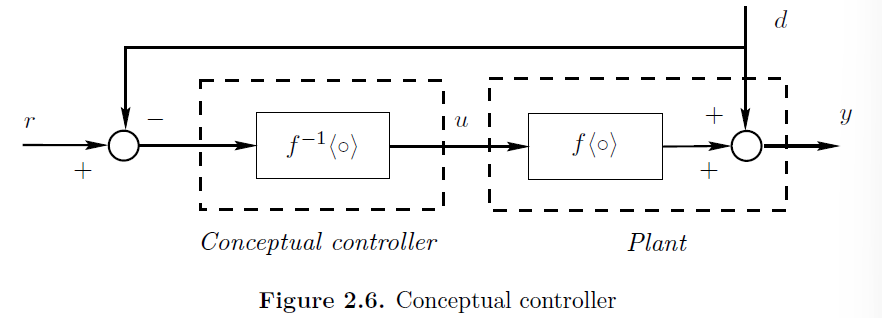
\includegraphics[width=3.54331in,height=1.27736in]{media/image1.png}

具体而言，假设输出参考由标量信号（参考量）\(r(t)\)指定，输出变量\(y(t)\)存在加性扰动\(d(t)\)，且仅有一个控制变量\(u(t)\)。可以给出上图所示的普适性框架，设\(f\)为描述对象输入-输出关系的变换映射（也称为模型）：

\[y = f\left\langle u \right\rangle + d\]

对于给定的目标可以求解控制律为：

\[u = f^{- 1}\left\langle r - d \right\rangle\]

上述求逆解法的严格条件为：

\begin{enumerate}
\def\labelenumi{\arabic{enumi}.}
\item
  \(f\)需要精确描述对象动态；
\item
  \(f\)需要定义良好（此处设为BIBO稳定），且\(f^{- 1}\)与之具有相同的稳定性条件；
\item
  扰动\(d\)需要可测量，以保证\(u\)可计算；
\item
  控制作用\(u\)物理可实现，且不违反约束。
\end{enumerate}

而自动控制理论的核心课题在于，如何通过改进控制架构，以更鲁棒的方式实现求逆，同时能够放宽上述严苛条件。在现实控制问题中，实际系统通常违反上述条件中的多条。在实际工程中，需要加上以下两条限定因素：

\begin{enumerate}
\def\labelenumi{\arabic{enumi}.}
\item
  参考信号\(r\)限定为特定类别，目标行为仅渐近达成；
\item
  寻求近似逆变换。
\end{enumerate}

本质上，所有控制器均在可行范围内隐式生成被控对象的逆，控制器之间的差异在于生成所需近似逆的机制不同{[}1{]}。经典的近似逆方法包括：（1）开环高增益控制；（2）闭环控制架构

\subsection{Marino等人的研究序列}\label{marinoux7b49ux4ebaux7684ux7814ux7a76ux5e8fux5217}

\section{线性系统输出调节}\label{ux7ebfux6027ux7cfbux7edfux8f93ux51faux8c03ux8282}

\begin{longtable}[]{@{}
  >{\raggedright\arraybackslash}p{(\linewidth - 0\tabcolsep) * \real{1.0000}}@{}}
\toprule\noalign{}
\begin{minipage}[b]{\linewidth}\raggedright
\textbf{线性系统的调节问题如下}：

\[\begin{aligned}
\dot{x} = & A_{c}x + bu + Pw,\ \ x \in \mathbf{R}^{n},u \in \mathbf{R} \\
\dot{w} = & Rw,\ \ w \in \mathbf{R}^{2m + 1} \\
e = & {C_{c}x - qw,\ \ y}_{r} = qw,\ \ y = C_{c}x,\ \ y,y_{r},e \in \mathbf{R}
\end{aligned}\]

干扰\(Pw\)和参考输出\(qw\)均由稳定的线性外系统\(R\)生成。

\textbf{要求}：设计仅由\(e\)驱动的反馈控制器，\(\forall x(0)\)，所有的信号都有界，且随着\(t \rightarrow \infty,\ \ e(t) \rightarrow \infty\)。问题有解的几个充要条件是：

（A1）外系统稳定（stable）：不失一般性假设外系统稳定：\(\mathfrak{R}\left( \lambda(R) \right) < 0\)

（A2）可稳性（stabilizable）：\(\left( A_{c},b \right)\)可稳：\(\mathfrak{R}(\lambda) < 0,\ \ rank\begin{bmatrix}
\lambda I - A_{c} & b
\end{bmatrix} < n\)；

（A3）可检测性（detectable）：\((A_{c},C_{c})\)可测：\(\mathfrak{R}(\lambda) < 0,\ \ rank\begin{bmatrix}
\lambda I - A_{c} \\
C_{c}
\end{bmatrix} < n\)

（A4）传输零点条件（Transmission zero
Condtion）：\(\forall\lambda(R),rank\left( \begin{bmatrix}
\lambda(R)I - A_{c} & b \\
C_{c} & 0
\end{bmatrix} \right) = n + 1\)，即此矩阵行满秩。换言之，\(R\)的特征值与系统传函的传输零点不重合。

\textbf{以上Assumption共同构成了线性输出调节问题有解的条件。}
\end{minipage} \\
\midrule\noalign{}
\endhead
\bottomrule\noalign{}
\endlastfoot
Marino和Tomei在其2003年的早期研究中已经涉足非标准的输出调节问题。研究不再要求完全掌握关于\(R\)的知识，而是利用一个在（A5）假设下使\textbf{自适应内模}指数收敛到\textbf{未知外系统}。

（A5）外系统\(R\)的特征值没有重根，并且分布在虚轴上；所有的振荡模态都能够由初始条件激励起来，并且这些振荡模态都能够从参考输入中观测到（observable）。

\(\begin{aligned}
\pi R = & A_{c}\pi + bc + P \\
q = & C_{c}\pi
\end{aligned}\)

方程的解为\((\pi,c)\)。*方程存在唯一解是由（A4）保证的。

结合这些假设，只需要外系统阶次的知识（要求初始条件能够激起所有的振荡模态）就可以做到输出调节。随后在Marino和San于2007年的研究中，这一假设被放松为阶次未知但其上限已知，研究使用间接自适应方法解决了这一问题，但控制较为复杂，这篇研究中将其简化。

（H1）能观性假设：被控系统\((A_{c},\ C_{c})\)能观；

（H2）最小相位假设：函数\(C_{c}adj\left( sI - A_{c} \right)^{- 1}\)的零点在LHP；

（H3）记外系统\(R\)的谱为\(\{ \pm j\omega_{i},\ \ 1 \leq i \leq m\}\)，其中\(\omega_{i}\)为未知参数，\(m\)为已知整数。由于最小相位假设，传输零点假设（A4）满足，调节方程\(\pi R = A_{c}\pi + b\gamma + P,q = c\pi\)的有解\((\pi,\gamma)\)且\((R,\gamma)\)能观 \\
\end{longtable}

\section{Marino2011理论基础}\label{marino2011ux7406ux8bbaux57faux7840}

在Marino和Tomei于2011年发表在Automatica的这篇文章里，没有将输出调节相关的理论做过多的阐述，仅引用了其结论。好在他们在2007年发表在TAC上的Output
Regulation for Linear Minimum Phase Systems With Unknown Order Exosystem
对这个话题作了比较详细的说明，我们才有了一个切入点，更喜人的是这篇文章中的表述与黄捷等人的研究表述基本一致，为我们的研究提供了较大的便利。

需要说明的是，尽管在阅读2011年这篇文献的同时参考了2007年的这篇文章。两者研究的问题并不相同。2007年所作假设是外系统阶次上限已知而外系统参数完全未知，到了2011年，这一假设修改为外系统阶次上限未知而外系统参数有界已知。需要注意研究者在处理这两种不同问题时所采取的控制器设计方法差异。

\begin{longtable}[]{@{}
  >{\raggedright\arraybackslash}p{(\linewidth - 0\tabcolsep) * \real{1.0000}}@{}}
\toprule\noalign{}
\begin{minipage}[b]{\linewidth}\raggedright
\textbf{鲁棒自适应学习调节问题}

系统参数向量有界：\(\alpha \in \Omega_{1} \subset \mathbf{R}^{2n - \rho + 1}\)

建模外系统参数向量有界：\(\overline{\theta} \in \Omega_{2} \subset \mathbf{R}^{\overline{m}}\)，球形边界半径为\(r_{\Omega_{2}}\)

自适应学习输出误差反馈系统：

\[\begin{aligned}
u = & f_{u}\left( v,\widehat{\theta},y - y_{r} \right) \\
\dot{v} = & f_{v}\left( v,\widehat{\theta},y - y_{r} \right),v(0) = v_{0},v \in \mathbf{R}^{S} \\
\dot{\widehat{\theta}} = & f_{\widehat{\theta}}\left( v,\widehat{\theta},y - y_{r} \right),\widehat{\theta}(0) = {\widehat{\theta}}_{0},\widehat{\theta} \in \mathbf{R}^{\overline{m}}
\end{aligned}\]

对于任意初始条件，所有闭环信号有界且

\begin{enumerate}
\def\labelenumi{\roman{enumi}.}
\item
  若\(\overline{m} < m\)（欠建模），\(\lbrack y(t) - y_{r}(t)\rbrack\)和\(\lbrack u(t) - u_{r}(t)\rbrack\)指数收敛到半径为关于\(\epsilon_{M}\)的class-k
  functions残差球体里；
\item
  若\(\overline{m} = m\)（完全建模），随着\(t \rightarrow \infty\)，\(\lbrack y(t) - y_{r}(t)\rbrack\)和\(\lbrack u(t) - u_{r}(t)\rbrack\)\textbf{指数收敛}到0；
\item
  若\(\overline{m} > m\)（过建模），
\end{enumerate}

\begin{quote}
\[\lim_{t \rightarrow \infty}{\left\lbrack y(t) - y_{r}(t) \right\rbrack = 0},\ \ \lim_{t \rightarrow \infty}{\left\lbrack u(t) - u_{r}(t) \right\rbrack = 0}\]
\end{quote}
\end{minipage} \\
\midrule\noalign{}
\endhead
\bottomrule\noalign{}
\endlastfoot
\textbf{线性能观最小相位系统}

\(\begin{aligned}
\dot{\overline{x}}\mathbf{= \&}A_{c}\overline{x} + a{\overline{x}}_{1} + \frac{1}{\beta}\overline{b}u + Pw,\ \ \overline{x} \in \mathbf{R}^{n},u \in \mathbf{R} \\
y = & C_{c}\overline{x},\ \ y \in \mathbf{R} \\
\dot{w} = & Rw,\ \ w \in \mathbf{R}^{2m + 1} \\
y_{r} = & qw
\end{aligned}\)

其中：

\(A_{c} = \begin{bmatrix}
0 & 1 & \ldots & 0 \\
 \vdots & \vdots & \ddots & \vdots \\
0 & 0 & \ldots & 1 \\
0 & 0 & \ldots & 0
\end{bmatrix},\ \ a = \begin{bmatrix}
a_{1} \\
 \vdots \\
a_{n - 1} \\
a_{n}
\end{bmatrix},\ \ \overline{b} = \begin{bmatrix}
0 \\
 \vdots \\
1 \\
{\overline{b}}_{\rho + 1} \\
 \vdots \\
{\overline{b}}_{n}
\end{bmatrix},\ \ C_{c} = \begin{bmatrix}
1 & 0 & \cdots & 0
\end{bmatrix}\)

这些参数共同构成有界的系统参数向量\(\alpha = \left\lbrack a_{1},\cdots,a_{n},\frac{1}{\beta},\ {\overline{b}}_{\rho + 1},\cdots,{\overline{b}}_{n} \right\rbrack^{\top}\)，\(\alpha \in \Omega_{1} \subset \mathbf{R}^{2n - \rho + 1}\)

假设外系统含有\(m\)个频率（\(m\)未知），矩阵\(R\)的特征多项式由\(s\Pi_{i = 1}^{m}\left( s^{2} + \omega_{i}^{2} \right) = s\left( s^{2m} + \theta_{1}s^{2m - 2} + \cdots + \theta_{m} \right)\)。估计外系统参数向量为\(\overline{\theta} \in \Omega_{2} \subset \mathbf{R}^{\overline{m}}\)

*为什么状态空间模型书写的形式是这样的特殊形式？为什么要分离\(x_{1},\beta?\) \\
\textbf{滤波变换}

对于阶次为\(n\)，相对阶为\(\rho\)的SISO系统，先引入一组输入滤波器状态\(\phi = \left\lbrack \phi_{1},\ldots,\phi_{\rho - 1} \right\rbrack^{\top}\)

\(\dot{\phi} = \begin{bmatrix}
 - \lambda_{1} & 1 & & 0 \\
 & - \lambda_{2} & \ddots & \vdots \\
 & & \ddots & 1 \\
0 & & & - \lambda_{\rho - 1}
\end{bmatrix}\phi + \begin{bmatrix}
0 \\
 \vdots \\
0 \\
1
\end{bmatrix}u,\ \ \phi(0) = 0\)

其中\(\lambda_{i} > 0\)为设计参数。这一组滤波器的作用是将信号\(\phi_{1}\)从原输入\(u\)中分离出来，这对于\(\rho \geq 2\)的系统自适应控制设计是必要的。

通过坐标变换\(x_{i} = {\overline{x}}_{i} - \frac{1}{\beta}\sum_{j = 2}^{\rho}{b_{i}\lbrack j\rbrack\phi_{j - 1}}\)，原系统状态\({\overline{x}}_{i}\)可以映射为新状态\(x_{i}\)

经过这一变换，上述系统变为

\(\begin{aligned}
\dot{x} = & A_{c}x + ay + \frac{1}{\beta}b\phi_{1} + Pw,\ \ x \in \mathbf{R}^{n},\phi_{1} \in \mathbf{R} \\
y = & C_{c}x,\ \ y \in \mathbf{R}
\end{aligned}\)

其中新参数\(b = h_{b}\left( \lambda,\overline{b} \right)。\)

*需要说明的是，在设计过程中对系统进行了这些变换，并不表示最终控制器中含有这些结构。 \\
\textbf{系统的非最小实现}

\(\begin{aligned}
\dot{x} = & A_{c}x + ay + \frac{1}{\beta}b\phi_{1} + Pw,\ \ x \in \mathbf{R}^{n},\phi_{1} \in \mathbf{R} \\
y = & C_{c}x,\ \ y \in \mathbf{R} \\
\dot{w} = & Rw,\ \ w \in \mathbf{R}^{2m + 1} \\
y_{r} = & qw \\
u_{r}/\phi_{1r} = & cw
\end{aligned}\)

其中向量\(b\)由\(\overline{b}\)与\(\lambda_{i},\ \ i = 1,\cdots,\rho - 1\)决定，当\(\rho = 1\)时二者完全等价。

这一非最小实现

（1）将信号\(\phi_{1}\)分离出来，对于自适应控制算法的设计是必要的；

（2）这一系统是能观的最小相位系统（因而也是能稳的）。 \\
\textbf{调节器矩阵方程}

\(\begin{aligned}
\pi R = & A_{c}\pi + aq + \frac{1}{\beta}bc + P \\
q = & C_{c}\pi
\end{aligned}\)

方程的解为\((\pi,c)\)

*满足Regulator
Eq的参数/根据方程解设计的参考信号\(x_{r} = \pi w,\ \ u_{r} = cw\)能够被渐进跟踪。 \\
\end{longtable}

出于某种原因？参考信号也可以直接建模为：

\[\begin{aligned}
{\dot{x}}_{r} = & A_{c}x_{r} + ay_{r} + \frac{1}{\beta}bu_{r} + Pw \\
y_{r} = & C_{c}x_{r} \\
u_{r}/\phi_{1r} = & cw
\end{aligned}\]

不失一般性地，可以考虑\((R,c)\)能观，且所有振荡模态都被激励起来的情况（对于不符合条件的情况，可以通过Kalman分解提取其中能观且模态能激励的部分）。

\[\begin{aligned}
{\dot{w}}_{c} = & R_{c}w_{c},\ \ w_{c} \in \mathbf{R}^{2m + 1} \\
u_{r}/\phi_{1r} = & \gamma_{c}w_{c} \\
R_{c} = \begin{bmatrix}
0 & 1 & 0 & \ldots & 0 \\
 - \theta_{1} & 0 & 1 & \ldots & 0 \\
 \vdots & \vdots & \vdots & \ddots & \vdots \\
 - \theta_{m} & 0 & 0 & \ldots & 1 \\
0 & 0 & 0 & \ldots & 0
\end{bmatrix},\ \ \gamma_{c} = \begin{bmatrix}
1 & 0 & \cdots & 0
\end{bmatrix}
\end{aligned}\]

*自适应学习控制的目标是仅基于调节误差的测量，通过``学习''控制参考输入\(u \rightarrow u_{r}\)达到驱动\(y \rightarrow y_{r}\)的目标。

\[\begin{aligned}
{\dot{\overline{w}}}_{c} = & {\overline{R}}_{c}{\overline{w}}_{c},\ \ w_{c} \in \mathbf{R}^{2\overline{m} + 1} \\
{\overline{u}}_{r}/{\overline{\phi}}_{1r} = & {\overline{\gamma}}_{c}{\overline{w}}_{c} \\
{\overline{R}}_{c} = \begin{bmatrix}
0 & 1 & 0 & \ldots & 0 \\
 - {\theta'}_{1} & 0 & 1 & \ldots & 0 \\
 \vdots & \vdots & \vdots & \ddots & \vdots \\
 - {\theta'}_{\overline{m}} & 0 & 0 & \ldots & 1 \\
0 & 0 & 0 & \ldots & 0
\end{bmatrix},\ \ {\overline{\gamma}}_{c} = \begin{bmatrix}
1 & 0 & \cdots & 0
\end{bmatrix}
\end{aligned}\]

剩余未建模的部分如下：

\[\begin{aligned}
{\dot{\overline{w}}}_{cr} = & {\overline{R}}_{cr}{\overline{w}}_{cr},\ \ w_{cr} \in \mathbf{R}^{2(m - \overline{m})} \\
r = & C_{c}{\overline{w}}_{cr} \\
{\overline{R}}_{c} = & \begin{bmatrix}
0 & 1 & 0 & \ldots & 0 \\
 - {\theta'}_{\overline{m} + 1} & 0 & 1 & \ldots & 0 \\
 \vdots & \vdots & \vdots & \ddots & \vdots \\
 - {\theta'}_{\overline{m}} & 0 & 0 & \ldots & 0
\end{bmatrix}
\end{aligned}\]

综上有：

\[u_{r}/\phi_{1r} = \gamma_{c}w_{c} = C_{c}({\overline{w}}_{c} + {\overline{w}}_{cr}) = {\overline{u}}_{r}/{\overline{\phi}}_{1r} + r\]

而误差模型有：

\[\begin{aligned}
\dot{\widetilde{x}} = & A_{c}\widetilde{x} + a({y - y}_{r}) + \frac{1}{\beta}b{(u - u}_{r}) \\
y - y_{r} = & C_{c}\widetilde{x}
\end{aligned}\]

记\(e = y - y_{r}\)，\(u_{r} = {\overline{u}}_{r} + r = {\overline{w}}_{c1} + r\)，则有：

\[\begin{aligned}
\dot{\widetilde{x}} = & A_{c}\widetilde{x} + ae + \frac{1}{\beta}b{(u - u}_{r}) \\
 = & A_{c}\widetilde{x} + ae + \frac{1}{\beta}b(u - {\overline{w}}_{c1} - r) \\
e = & C_{c}\widetilde{x}
\end{aligned}\]

\subsection{ρ=1的鲁棒自适应学习调节}\label{ux3c11ux7684ux9c81ux68d2ux81eaux9002ux5e94ux5b66ux4e60ux8c03ux8282}

被控系统建模如下：

\[\begin{aligned}
\dot{x} = & A_{c}x + ay + \frac{1}{\beta}b\phi_{1} + Pw \\
y = & C_{c}x \\
y_{r} = & qw
\end{aligned}\]

外系统（干扰与参考信号）建模如下：

\[\begin{aligned}
{\dot{w}}_{c} = & R_{c}w_{c},\ \ w_{c} \in \mathbf{R}^{2m + 1} \\
u_{r} = & \gamma_{c}w_{c} \\
R_{c} = \begin{bmatrix}
0 & 1 & 0 & \ldots & 0 \\
 - \theta_{1} & 0 & 1 & \ldots & 0 \\
 \vdots & \vdots & \vdots & \ddots & \vdots \\
 - \theta_{m} & 0 & 0 & \ldots & 1 \\
0 & 0 & 0 & \ldots & 0
\end{bmatrix},\ \ \gamma_{c} = \begin{bmatrix}
1 & 0 & \cdots & 0
\end{bmatrix}
\end{aligned}\]

\begin{longtable}[]{@{}
  >{\raggedright\arraybackslash}p{(\linewidth - 0\tabcolsep) * \real{1.0000}}@{}}
\toprule\noalign{}
\begin{minipage}[b]{\linewidth}\raggedright
设计控制器如下：

\[u = - {\widehat{\chi}}_{1} - \mu^{\top}{\widehat{\theta}}_{1} - k\left( y - y_{r} \right)\]

未知状态的观测器：

\[\dot{\widehat{\chi}} = D\widehat{\chi} - \overline{d}u,\ \ \widehat{\chi} \in \mathbf{R}^{2\overline{m} + 1}\]

其中\(D\)是一个大小合适的Hurwitz矩阵，而\(d\)是一个由系数构成的常向量，通常可取：

\[D = \ \begin{bmatrix}
 - d_{2} & 1 & 0 & 0 \\
 - d_{3} & 0 & 1 & 0 \\
 - d_{4} & 0 & 0 & 1 \\
 - d_{5} & 0 & 0 & 0
\end{bmatrix}\]

外系统未知参数\(\theta\)（此处取频率参数）的估计值：

\[\begin{array}{r}
\dot{\widehat{\theta}} = g \cdot Proj\left( \mu\left( y - y_{r} \right),\widehat{\theta} \right)
\end{array},\ \ \widehat{\theta} \in \mathbf{R}^{\overline{m}}\]

其中：

\[\begin{aligned}
{\dot{\xi}}_{i} = & D\xi_{i} + \left\lbrack 0\ I_{2\overline{m} + 1} \right\rbrack E_{2i + 1}u,\ \ \xi_{i} \in \mathbf{R}^{2\overline{m} + 1} \\
\mu_{i} = & \lbrack 1\ 0\cdots 0\rbrack\xi_{i},\ \ 1 \leq i \leq \overline{m}
\end{aligned}\]
\end{minipage} \\
\midrule\noalign{}
\endhead
\bottomrule\noalign{}
\endlastfoot
\textbf{Remark 1}

对于\(u(t) \rightarrow \mu_{i}(t),\ \ 1 \leq i \leq \overline{m}\)的线性滤波器；

观测器有\({\widehat{\chi}}_{1}(t)\)的最小实现阶次为\(2\overline{m} + 1\)；

所涉及的动态控制器阶次为\(3\overline{m} + 1\) \\
\textbf{Remark
2}考虑一种简化情况：外系统参数\(\theta\)参数完全已知，\(\overline{m} = m\)，

则可以将以上\(\widehat{\theta}\)替换为\(\theta\)，控制算法变为一个由\(\theta\)线性参数化的补偿器；

这一线性参数化对于涉及自适应控制器至关重要。 \\
\end{longtable}

\subsection{ρ≥2的鲁棒自适应学习调节}\label{ux3c12ux7684ux9c81ux68d2ux81eaux9002ux5e94ux5b66ux4e60ux8c03ux8282}

ρ\textgreater1的方程及响应的自适应学习调节有所不同，这里用红色字体以示区分。

被控系统建模如下：

\[\begin{aligned}
\dot{x} = & A_{c}x + ay + \frac{1}{\beta}b\phi_{1} + Pw \\
y = & C_{c}x \\
y_{r} = & qw
\end{aligned}\]

外系统（干扰与参考信号）建模如下：

\[\begin{aligned}
\dot{w} = & Rw \\
x_{r} = & \pi w \\
\phi_{1r} = & cw
\end{aligned}\]

或者直接建模参考信号为：

\[\begin{aligned}
{\dot{x}}_{r} = & A_{c}x_{r} + ay_{r} + \frac{1}{\beta}b\phi_{1r} + Pw \\
y_{r} = & C_{c}x_{r} \\
\phi_{1r} = & cw \\
u_{r} = & \sum_{i = 1}^{\rho}{\delta_{\rho - i}\frac{d^{i - 1}\phi_{1r}(t)}{dt^{i - 1}}}
\end{aligned}\]

其中\(\delta_{0} = 1,\ \ \delta_{i},\ 1 \leq i \leq \rho - 1\)为以下模型的系数：

\[\Pi_{i = 1}^{\rho - 1}\left( s + \lambda_{i} \right) = \sum_{i = 1}^{\rho}{\delta_{\rho - i}s^{i - 1}}\]

而将干扰建模为：

\[\begin{aligned}
{\dot{w}}_{c} = & R_{c}w_{c},\ \ w_{c} \in \mathbf{R}^{2m + 1} \\
\phi_{1r} = & \gamma_{c}w_{c} \\
R_{c} = \begin{bmatrix}
0 & 1 & 0 & \ldots & 0 \\
 - \theta_{1} & 0 & 1 & \ldots & 0 \\
 \vdots & \vdots & \vdots & \ddots & \vdots \\
 - \theta_{m} & 0 & 0 & \ldots & 1 \\
0 & 0 & 0 & \ldots & 0
\end{bmatrix},\ \ \gamma_{c} = \begin{bmatrix}
1 & 0 & \cdots & 0
\end{bmatrix}
\end{aligned}\]

\begin{longtable}[]{@{}
  >{\raggedright\arraybackslash}p{(\linewidth - 0\tabcolsep) * \real{1.0000}}@{}}
\toprule\noalign{}
\begin{minipage}[b]{\linewidth}\raggedright
设计控制器如下：

\[\begin{array}{r}
u = \lambda_{1}\phi_{1}^{*} - {\dot{\widehat{\chi}}}_{1} - {\dot{\mu}}^{\top}\widehat{\theta} - \mu^{\top}\dot{\widehat{\theta}} \\
\phi_{1}^{*} = - {\widehat{\chi}}_{1} - \mu^{\top}{\widehat{\theta}}_{1} - k\left( y - y_{r} \right)
\end{array}\]

未知状态的观测器：

\[\dot{\widehat{\chi}} = D\widehat{\chi} - \overline{d}\phi_{1},\ \ \widehat{\chi} \in \mathbf{R}^{2\overline{m} + 1}\]

其中\(D\)是一个大小合适的Hurwitz矩阵，而\(d\)是一个由系数构成的常向量，通常可取：

\[D = \begin{bmatrix}
 - d_{2} & 1 & 0 & 0 \\
 - d_{3} & 0 & 1 & 0 \\
 - d_{4} & 0 & 0 & 1 \\
 - d_{5} & 0 & 0 & 0
\end{bmatrix}\]

外系统未知参数\(\theta\)（此处取频率参数）的估计值：

\[\begin{array}{r}
\dot{\widehat{\theta}} = g \cdot Proj\left( \mu\left( y - y_{r} \right),\widehat{\theta} \right)
\end{array},\ \ \widehat{\theta} \in \mathbf{R}^{\overline{m}}\]

其中：

\[\begin{aligned}
{\dot{\xi}}_{i} = & D\xi_{i} + \left\lbrack 0\ I_{2\overline{m} + 1} \right\rbrack E_{2i + 1}\phi_{1},\ \ \xi_{i} \in \mathbf{R}^{2\overline{m} + 1} \\
\mu_{i} = & \lbrack 1\ 0\cdots 0\rbrack\xi_{i},\ \ 1 \leq i \leq \overline{m}
\end{aligned}\]
\end{minipage} \\
\midrule\noalign{}
\endhead
\bottomrule\noalign{}
\endlastfoot
\end{longtable}

\subsection{ρ=1仿真复现}\label{ux3c11ux4effux771fux590dux73b0}

\subsubsection{被控系统、外系统建模}\label{ux88abux63a7ux7cfbux7edfux5916ux7cfbux7edfux5efaux6a21}

被控系统建模如下：

\[\begin{aligned}
{\dot{x}}_{1} = & x_{2} + a_{1}x_{1} + \frac{1}{\beta}u + w_{1} \\
{\dot{x}}_{2} = & \frac{1}{\beta}b_{2}u \\
y = & x_{1}
\end{aligned}\]

参考输出为：

\[y_{r} = - w_{2}\]

外系统建模如下：

\[P{w(t) = w}_{1}(t) = \left\{ \begin{array}{r}
\sin{\omega_{1}t} + 0.2\sin{\omega_{3}t},\ \ t < 50s \\
\sin{\omega_{1}t},\ \ t \geq 50s
\end{array} \right.\ \]

\[- qw = w_{2}(t) = \left\{ \begin{array}{r}
\sin{\omega_{2}t},\ \ t < 100s \\
0,\ \ t \geq 100s
\end{array} \right.\ \]

*仿真中直接建模\(w_{1},w_{2}\)，而在此前理论部分所用符号为\(w_{c},{\overline{w}}_{c},w_{c1},{\overline{w}}_{c1}\)等。这些不同符号之间有何关系？

\subsubsection{控制器设计}\label{ux63a7ux5236ux5668ux8bbeux8ba1}

控制器目标有如下三个：

\begin{enumerate}
\def\labelenumi{\arabic{enumi}.}
\item
  使系统输出\(y = x_{1}\)渐进跟踪参考输出\(y_{r} = - w_{2}\)；
\item
  保证所有内部信号有界；
\item
  估计未知参数。
\end{enumerate}

参照前文，设计控制器如下：

\[u = - ke - {\widehat{\chi}}_{1} - \mu_{1}{\widehat{\theta}}_{1} - \mu_{2}{\widehat{\theta}}_{2}\]

未知状态的观测器：

\[\dot{\widehat{\chi}} = D\widehat{\chi} - \left\lbrack d_{2}\ d_{3}\ d_{4}\ d_{5} \right\rbrack^{\top}u\]

其中：

\[D = \ \begin{bmatrix}
 - d_{2} & 1 & 0 & 0 \\
 - d_{3} & 0 & 1 & 0 \\
 - d_{4} & 0 & 0 & 1 \\
 - d_{5} & 0 & 0 & 0
\end{bmatrix}\]

外系统未知参数\(\theta_{1},\theta_{2}\)（此处取频率参数）的估计值：

\[\begin{aligned}
{\widehat{\theta}}_{1} = & g \cdot Proj\left( \mu_{1}e,{\widehat{\theta}}_{1} \right) \\
{\widehat{\theta}}_{2} = & g \cdot Proj\left( \mu_{2}e,{\widehat{\theta}}_{2} \right)
\end{aligned}\]

其中：

\[\begin{aligned}
{\dot{\xi}}_{1} = & D\xi_{1} + \lbrack 0\ u\ 0\ 0\rbrack^{\top} \\
{\dot{\xi}}_{2} = & D\xi_{2} + \lbrack 0\ 0\ 0\ u\rbrack^{\top} \\
\mu_{1} = \xi_{11},\ \ \mu_{2} = \xi_{21}
\end{aligned}\]

\subsubsection{仿真}\label{ux4effux771f}

在程序中，状态矩阵X通过ODE45求解得到，共有16列，每一列代表系统中的一个状态变量。具体解释如下：

\begin{longtable}[]{@{}
  >{\raggedright\arraybackslash}p{(\linewidth - 0\tabcolsep) * \real{1.0000}}@{}}
\toprule\noalign{}
\begin{minipage}[b]{\linewidth}\raggedright
x = X(1:2); \% 系统状态 {[}x1; x2{]}

xi1 = X(3:6); \% 滤波器ξ1状态

xi2 = X(7:10); \% 滤波器ξ2状态

chi\_hat = X(11:14); \% 估计器χ状态

theta\_hat = X(15:16); \% 参数估计 {[}θ1\_hat; θ2\_hat{]}
\end{minipage} \\
\midrule\noalign{}
\endhead
\bottomrule\noalign{}
\endlastfoot
\end{longtable}

\begin{enumerate}
\def\labelenumi{\arabic{enumi}.}
\item
  第1\textasciitilde2列依次代表系统状态\(x_{1},\ \ x_{2}\)；
\item
  第3\textasciitilde6列代表滤波器状态\(\xi_{1} = \left\lbrack \xi_{11}\ \xi_{12}\ \xi_{13}\ \xi_{14} \right\rbrack^{\top}\)，其中\(\mu_{1} = \xi_{11}\)；
\item
  第7\textasciitilde10列代表滤波器状态\(\xi_{2} = \left\lbrack \xi_{21}\ \xi_{22}\ \xi_{23}\ \xi_{24} \right\rbrack^{\top}\)，其中\(\mu_{2} = \xi_{21}\)；
\item
  第11\textasciitilde14列代表观测器状态\(\widehat{\chi} = \left\lbrack {\widehat{\chi}}_{1}\ {\widehat{\chi}}_{2}\ {\widehat{\chi}}_{3}\ {\widehat{\chi}}_{4} \right\rbrack^{\top}\)，其中\({\widehat{\chi}}_{1}\)直接用于控制律；
\item
  第15\textasciitilde16列代表参数估计\(\widehat{\theta} = \left\lbrack {\widehat{\theta}}_{1}\ {\widehat{\theta}}_{2} \right\rbrack^{\top}\)。
\end{enumerate}

\subsubsection{仿真案例分析}\label{ux4effux771fux6848ux4f8bux5206ux6790}

\begin{enumerate}
\def\labelenumi{\arabic{enumi}.}
\item
  外系统模型与干扰/参考信号之间的关系
\item
  控制器设计的逻辑
\end{enumerate}

\begin{quote}
控制器\(u\)最终仅由输入\(u\)与误差\(e\)驱动，控制器结构含有观测器等诸多因素，相对复杂。
\end{quote}

\subsection{ρ≥2算法仿真}\label{ux3c12ux7b97ux6cd5ux4effux771f}

\subsection{小结}\label{ux5c0fux7ed3}

文章的表述过于数学化，我希望能够将其``翻译''为具有更强物理/信息意义的表达。这就涉及到探讨以下的一些问题。

\begin{enumerate}
\def\labelenumi{\arabic{enumi}.}
\item
  文章是通过什么方式来实现抗干扰的？
\item
  文章是通过什么方式来实现渐进跟踪的？
\item
  对被控对象和外系统作了哪些假设？
\item
  控制器设计用到了哪些信息？
\item
  自适应部分还能否看作是参数自适应？还是否对应于某些特定的从参数自适应算法？
\end{enumerate}

更具体的问题如下：

\begin{enumerate}
\def\labelenumi{\arabic{enumi}.}
\item
  控制律\(u\)的各部分构成应该如何理解？
\item
  文章提到\(\chi\)是一个observer，但它是对什么的观测？
\item
  \(\xi\)是一个仅由\(u\)为输入的系统的状态变量，\(\mu\)是它的输出（regressor），这是否构成一个固定控制器？
\item
  \(\widehat{\theta}\)是一个由误差\(e\)直接驱动，由\(u\)间接驱动的内模参数自适应估计，并且作为了regressor
  \(\mu\)的参数。
\end{enumerate}

2015年至今开启了Marino等人研究的第三阶段，这一阶段的研究假设被控对象系统未知，外系统阶次已知但参数未知，持续为输出调节问题的最简先验假设探究提出新的问题。一般认为Pigg和Bodson在2010年的研究打下了早期基础；Marino与Tomei于2011年最早研究了被控对象不完全已知（最小相位且相对阶已知）且外系统不确定的问题。2015年设计固定控制器，并于2016年将其用于设计自适应控制器。

\begin{longtable}[]{@{}
  >{\raggedright\arraybackslash}p{(\linewidth - 6\tabcolsep) * \real{0.0895}}
  >{\raggedright\arraybackslash}p{(\linewidth - 6\tabcolsep) * \real{0.3026}}
  >{\raggedright\arraybackslash}p{(\linewidth - 6\tabcolsep) * \real{0.3054}}
  >{\raggedright\arraybackslash}p{(\linewidth - 6\tabcolsep) * \real{0.3026}}@{}}
\toprule\noalign{}
\begin{minipage}[b]{\linewidth}\raggedright
\textbf{维度}
\end{minipage} & \begin{minipage}[b]{\linewidth}\raggedright
\textbf{Theorem 3.1}
\end{minipage} & \begin{minipage}[b]{\linewidth}\raggedright
\textbf{Theorem 3.2}
\end{minipage} & \begin{minipage}[b]{\linewidth}\raggedright
\textbf{Theorem 3.3}
\end{minipage} \\
\midrule\noalign{}
\endhead
\bottomrule\noalign{}
\endlastfoot
\textbf{系统模型 P(s)} & 稳定的有理传递函数，且 P(0)≠0，Re{[}P(jωi){]}
或 Im{[}P(jωi){]} 非零且符号已知 & 稳定的有理传递函数，且 Re{[}P(jω){]}
\textgreater{} 0 对所有 ω ∈ R 成立 & 稳定的有理传递函数，且
P(0)≠0，Re{[}P(jωi){]} 或 Im{[}P(jωi){]} 非零且符号已知 \\
\textbf{外系统/干扰建模} & 干扰为已知频率的偏置多正弦信号 &
干扰为已知频率的偏置多正弦信号 & 干扰为已知频率的偏置多正弦信号 \\
\textbf{动态补偿器阶数} & 2q +1 & 2q +1 & 2q +1 \\
\textbf{频率数量已知性} & 已知干扰中正弦分量的频率 ωi，1 ≤i ≤q &
已知干扰中正弦分量的频率 ωi，1 ≤i ≤q & 已知干扰中正弦分量的频率 ωi，1 ≤i
≤q \\
\textbf{设计目标} &
设计动态输出反馈控制器，解决调节器问题，即抵消偏置多正弦扰动 &
设计动态输出反馈控制器，解决调节器问题，即抵消偏置多正弦扰动 &
设计动态输出反馈控制器，解决调节器问题，即抵消偏置多正弦扰动 \\
\textbf{自适应策略} & 无 & 无 & 无 \\
\textbf{关键假设} & P(0) 的符号已知，且对于每个频率 ωi，Re{[}P(jωi){]}
或 Im{[}P(jωi){]} 的符号已知 & Re{[}P(jω){]} \textgreater{} 0 对所有 ω ∈
R 成立，且干扰频率已知 & P(0) 的符号已知，且对于每个频率
ωi，Re{[}P(jωi){]} 或 Im{[}P(jωi){]} 的符号已知 \\
\textbf{主要结论} &
在控制增益足够小的情况下，所设计的动态输出反馈控制器能够解决调节器问题 &
对于任何有限正增益 k \textgreater{}
0，所设计的动态输出反馈控制器能够解决调节器问题 &
在控制增益足够小的情况下，所设计的动态输出反馈控制器能够解决调节器问题 \\
\end{longtable}

\begin{longtable}[]{@{}
  >{\raggedright\arraybackslash}p{(\linewidth - 6\tabcolsep) * \real{0.1104}}
  >{\raggedright\arraybackslash}p{(\linewidth - 6\tabcolsep) * \real{0.3028}}
  >{\raggedright\arraybackslash}p{(\linewidth - 6\tabcolsep) * \real{0.3476}}
  >{\raggedright\arraybackslash}p{(\linewidth - 6\tabcolsep) * \real{0.2392}}@{}}
\toprule\noalign{}
\begin{minipage}[b]{\linewidth}\raggedright
\textbf{特征}
\end{minipage} & \begin{minipage}[b]{\linewidth}\raggedright
\textbf{Theorem 1}
\end{minipage} & \begin{minipage}[b]{\linewidth}\raggedright
\textbf{Theorem 2}
\end{minipage} & \begin{minipage}[b]{\linewidth}\raggedright
\textbf{Theorem 3（陷波器设计）}
\end{minipage} \\
\midrule\noalign{}
\endhead
\bottomrule\noalign{}
\endlastfoot
\textbf{系统模型P(s)} &
\multicolumn{2}{>{\raggedright\arraybackslash}p{(\linewidth - 6\tabcolsep) * \real{0.6504} + 2\tabcolsep}}{%
单输入单输出线性系统，稳定（所有极点实部为负），严格真，未知阶数和相对阶，只需知道传递函数在零频率及（所有）干扰频率处的实部或虚部的符号}
& 假设P(s)=1，即系统为纯积分器 \\
\textbf{外系统/干扰建模} &
干扰是单频偏置正弦波信号，具有未知偏置、频率、幅度和相位 &
干扰是多频偏置正弦波信号，具有未知偏置、多个未知频率、幅度和相位 &
干扰是多频偏置正弦波信号，具有未知偏置、多个未知频率、幅度和相位 \\
\textbf{动态补偿器阶数} & 4阶动态输出反馈补偿器 &
2q+1阶动态输出反馈补偿器（q为干扰频率数量） &
2q+1阶动态估计器（q为干扰频率数量） \\
\textbf{频率数量已知性} &
\multicolumn{3}{>{\centering\arraybackslash}p{(\linewidth - 6\tabcolsep) * \real{0.8896} + 4\tabcolsep}@{}}{%
假设干扰频率数量已知} \\
\textbf{设计目标} &
设计自适应补偿器，使系统输出和频率估计误差指数收敛至零 &
设计自适应补偿器，使系统输出和频率估计误差指数收敛至零 &
设计较动器，直接估计测量信号中的所有未知频率 \\
\textbf{自适应策略} &
\multicolumn{3}{>{\centering\arraybackslash}p{(\linewidth - 6\tabcolsep) * \real{0.8896} + 4\tabcolsep}@{}}{%
自适应调整频率估计值} \\
\textbf{关键假设} &
\multicolumn{2}{>{\centering\arraybackslash}p{(\linewidth - 6\tabcolsep) * \real{0.6504} + 2\tabcolsep}}{%
传递函数在（所有）干扰频率处的实部或虚部的符号已知} & 无 \\
\textbf{主要结论} &
\multicolumn{2}{>{\raggedright\arraybackslash}p{(\linewidth - 6\tabcolsep) * \real{0.6504} + 2\tabcolsep}}{%
在初始误差足够小的条件下，补偿器保证系统输出和频率估计误差的局部指数收敛}
&
在初始误差足够小的条件下，估计器保证频率估计误差的局部指数收敛，并提供频率估计值 \\
\end{longtable}

\section{Marino2013理论基础}\label{marino2013ux7406ux8bbaux57faux7840}

2013年的研究是Marino与Tomei重要的系列研究中最后一篇被控对象完全已知的。

\begin{longtable}[]{@{}
  >{\raggedright\arraybackslash}p{(\linewidth - 0\tabcolsep) * \real{1.0000}}@{}}
\toprule\noalign{}
\begin{minipage}[b]{\linewidth}\raggedright
\textbf{线性系统的调节问题如下}：

\[\begin{aligned}
\dot{x} = & Ax + bu + Pw,\ \ x \in \mathbf{R}^{n},u \in \mathbf{R} \\
\dot{w} = & Rw,\ \ w \in \mathbf{R}^{2r + 1} \\
e = & {cx + qw,\ \ y}_{r} = - qw,\ \ y = cx,\ \ y,y_{r},e \in \mathbf{R}
\end{aligned}\]

干扰\(Dz\)和参考输出\(- qz\)均由线性外系统\(R\)生成。

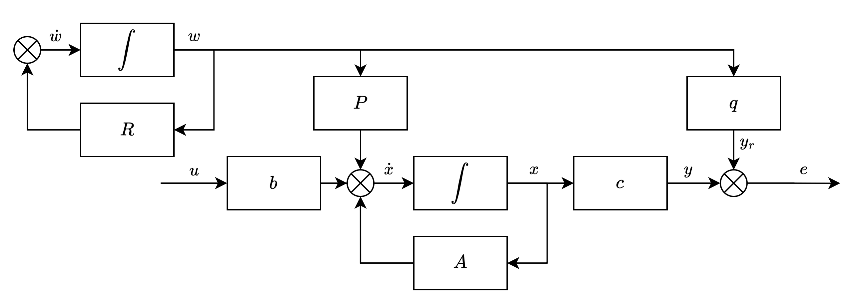
\includegraphics[width=3.93601in,height=1.38882in]{media/image2.png}

\textbf{要求}：设计仅由\(e\)驱动的反馈控制器，\(\forall x(0)\)，所有的信号都有界，且随着\(t \rightarrow \infty,\ \ e(t) \rightarrow 0\)。问题有解的几个充要条件是：

（A1）外系统不稳定（unstable）：不失一般性假设外系统不稳定：\(\mathfrak{R}\left( \lambda(R) \right) \geq 0\)

（A2）可稳性（stabilizable）：\((A,b)\)可稳：\(\mathfrak{R}(\lambda) < 0,\ \ rank\begin{bmatrix}
\lambda I - A & b
\end{bmatrix} < n\)；

（A3）可检测性（detectable）：\((A,c)\)可测：\(\mathfrak{R}(\lambda) < 0,\ \ rank\begin{bmatrix}
\lambda I - A \\
c
\end{bmatrix} < n\)

（A4）传输零点条件（Transmission zero
Condtion）：\(\forall\lambda(R),rank\left( \begin{bmatrix}
\lambda(R)I - A & b \\
c & 0
\end{bmatrix} \right) = n + 1\)，即此矩阵行满秩。换言之，\(R\)的特征值与系统传函的传输零点不重合。

\textbf{以上Assumption共同构成了线性输出调节问题有解的条件。}更具体地说，（A2）和（A3）构成系统可以通过误差反馈补偿镇定的条件；（A4）构成外系统可以从调节误差中观察到、干扰可以由控制器产生的条件。
\end{minipage} \\
\midrule\noalign{}
\endhead
\bottomrule\noalign{}
\endlastfoot
\end{longtable}

注意输出调节问题有解的上述假设并不强制要求被控对象\((A,b,c) ≔ P(s)\)为最小相位的（既不要求所有极点在LHP，也不要求零点在LHP），只需要满足（A4）规定的传输零点条件即可。

若外系统参数\(R,D,r\)完全已知，则根据内模原理可以给出调节器的设计。

\begin{longtable}[]{@{}
  >{\raggedright\arraybackslash}p{(\linewidth - 0\tabcolsep) * \real{1.0000}}@{}}
\toprule\noalign{}
\begin{minipage}[b]{\linewidth}\raggedright
\textbf{调节方程（Regulator Eq.）}

在上述条件下，以下调节方程存在唯一解\((\Gamma,\ \gamma)\)：

\[\Gamma R = A\Gamma + b\gamma + P\]

\[c\Gamma + q = 0\]

其中\(\Gamma \in \mathbf{R}^{n \times (2r + 1)}\)，\(\gamma \in \mathbf{R}^{1 \times (2r + 1)}\)

此时令\(x_{r} = \Gamma w\)，\(u_{r} = \gamma w\)，则得到：

\[\begin{aligned}
{\dot{x}}_{r} = & \Gamma(Rz) = Ax_{r} + bu_{r} + Pz \\
e = & cx_{r} + qw = 0
\end{aligned}\]

据此，调节问题可转化为\textbf{增广系统}的误差反馈镇定问题。

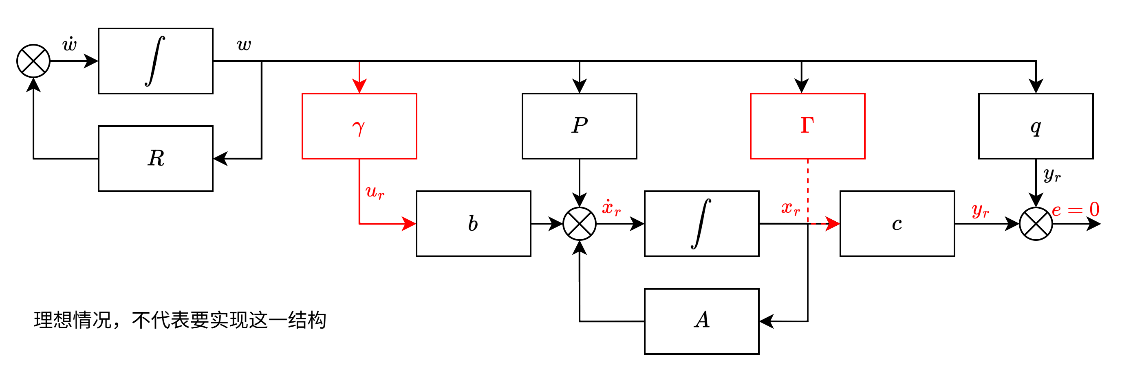
\includegraphics[width=5.12169in,height=1.67826in]{media/image3.png}
\end{minipage} \\
\midrule\noalign{}
\endhead
\bottomrule\noalign{}
\endlastfoot
按照LORP\textbf{状态反馈}控制解的流程，依次需要（1）设计反馈增益\(k_{c}\)使得\((A + bk_{c})\)Hurwitz；（2）求解Regulator
Equation得到\((\Gamma,\ \gamma)\)；（3）根据Regulator的解反解需要的\(k_{v}\)。

但由于exogenous signal显然不可直接测得/不可用于反馈，状态反馈不适用。

按照LORP\textbf{输出反馈}控制解的流程，依次需要（1）设计反馈增益\(k_{c}\)使得\((A + bk_{c})\)Hurwitz；（2）设计增广系统\((\overline{A},\ \overline{b},\overline{c})\)的状态观测器\(k_{o}\)使\((\overline{A} - k_{o}\overline{c})\)Hurwitz；（3）求解Regulator
Equation得到\((\Gamma,\ \gamma)\)；（3）根据Regulator的解反解需要的\(k_{v}\)；（4）根据反馈增益、前馈增益、状态观测重构反馈控制器的状态矩阵。 \\
\end{longtable}

\subsection{主要问题的转变}\label{ux4e3bux8981ux95eeux9898ux7684ux8f6cux53d8}

相对复杂深入的理论通常有这样的特点，使用数学工具对原有问题的细节进行分析。由此将原本定义良好的问题转换为另一个问题的探究。线性系统输出调节理论就具有这样的特点。对于以上给定的线性系统，理论说明，当干扰与参考输出可以由线性外系统\(R\)生成时，对于完整的增广系统，线性系统镇定、跟踪和抗干扰问题是否有解可由一系列充要条件判定。同样的，在Marino和Tomei的这篇文章中，同样将所要探究的主要问题进行了多次转变。

\begin{enumerate}
\def\labelenumi{\arabic{enumi}.}
\item
  \textbf{经典理论：}线性系统的输出调节问题↔增广系统Regulator
  Equation的可解性；
\item
  \textbf{构造误差系统}：\(y \rightarrow y_{r}\)输出调节问题↔系统控制+\(v \rightarrow u_{r}\)输入匹配与\(u_{r}\)合成问题；

  \begin{enumerate}
  \def\labelenumii{\alph{enumii})}
  \item
    设计状态反馈：\(u = k_{c}x + v\)
  \item
    设计输入\(v \rightarrow u_{r} = \gamma w\)：\(v = u_{rE}\)；
  \end{enumerate}
\end{enumerate}

\begin{quote}
\(u_{r}\)定义为理想能观标准型外系统的输出，\(u_{rE}\)是近似外系统的输出并且直接取\(v = u_{rE}\)；
\end{quote}

\begin{enumerate}
\def\labelenumi{\arabic{enumi}.}
\setcounter{enumi}{2}
\item
  \textbf{状态观测与反馈控制}：获取控制输入→Kalman分解、设计观测器增益\(k_{o}\)、状态反馈增益\(k_{c}\)
\item
  \textbf{参数化内模观测}：估计内模输出\(v = u_{rE} = \eta_{E1}\)

  \begin{enumerate}
  \def\labelenumii{\alph{enumii})}
  \item
    \textbf{构造观测器标准型}：对实际耦合系统进行线性变换，构造观测器标准型；
  \item
    \textbf{基于滤波变换的内模自适应}：通过滤波构造回归向量等，便于应用参数自适应算法进行参数估计，对滤波变换系统进行自适应观测。
  \end{enumerate}
\end{enumerate}

\subsection{参数化理想内模、理想耦合系统}\label{ux53c2ux6570ux5316ux7406ux60f3ux5185ux6a21ux7406ux60f3ux8026ux5408ux7cfbux7edf}

按照上述逻辑，构建误差系统将设计调节控制器的问题转变为设计\(v\)使得\(v\)收敛于\(u_{r} = c_{c}\eta\)的问题。其中\(u_{r} = c_{c}\eta\)是参数化外系统模型的输出，假定外系统模型\(R_{c}\)结构已知，参数未知。

\begin{longtable}[]{@{}
  >{\raggedright\arraybackslash}p{(\linewidth - 0\tabcolsep) * \real{1.0000}}@{}}
\toprule\noalign{}
\begin{minipage}[b]{\linewidth}\raggedright
\textbf{误差系统}

令\(\widetilde{x} = x - x_{r}\)

\[\begin{aligned}
\dot{\widetilde{x}} = & A\widetilde{x} + b(u - u_{r}),\ \ u_{r} = \gamma w,\ \ x \in \mathbf{R}^{n},u \in \mathbf{R} \\
\dot{w} = & Rw,\ \ w \in \mathbf{R}^{2r + 1} \\
e = & {c\widetilde{x},\ \ y}_{r} = - qw,\ \ y = cx,\ \ y,y_{r},e \in \mathbf{R}
\end{aligned}\]

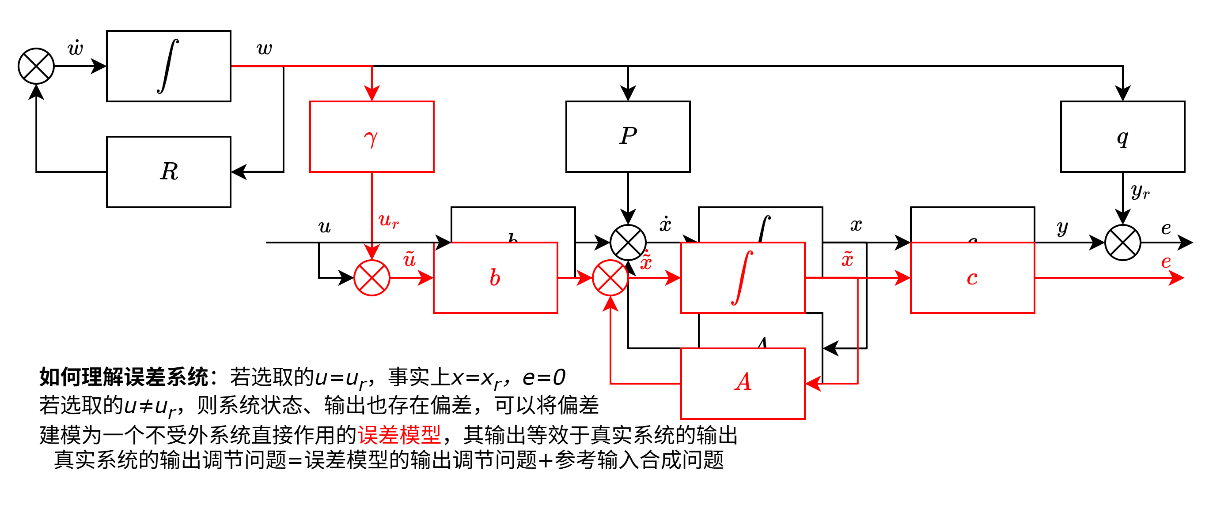
\includegraphics[width=5.54388in,height=2.296in]{media/image4.png}
\end{minipage} \\
\midrule\noalign{}
\endhead
\bottomrule\noalign{}
\endlastfoot
\textbf{Kalman分解能观子系统}

对被控系统进行Kalman分解\(\begin{bmatrix}
{\widetilde{x}}_{u} \\
{\widetilde{x}}_{o}
\end{bmatrix} = T_{1}\widetilde{x}\)：

\(\begin{aligned}
\begin{bmatrix}
{\dot{\widetilde{x}}}_{u} \\
{\dot{\widetilde{x}}}_{o}
\end{bmatrix} = & \begin{bmatrix}
A_{u} & A_{uo} \\
0 & A_{o}
\end{bmatrix}\begin{bmatrix}
{\widetilde{x}}_{u} \\
{\widetilde{x}}_{o}
\end{bmatrix} + \begin{bmatrix}
b_{u} \\
b_{o}
\end{bmatrix}(u - u_{r}),\ \ u_{r} = \gamma w,\ \ x \in \mathbf{R}^{n},u \in \mathbf{R} \\
e = & {\begin{bmatrix}
0 & c_{o}
\end{bmatrix}\begin{bmatrix}
{\widetilde{x}}_{u} \\
{\widetilde{x}}_{o}
\end{bmatrix},\ \ y}_{r} = - qw,\ \ y = cx,\ \ y,y_{r},e \in \mathbf{R}
\end{aligned}\)

其中\((A_{o},b_{o},c_{o})\)为能观标准型。 \\
\textbf{参数化理想内模}

将外系统\(\dot{w} = Rw,\ \ u_{r} = \gamma w\)重新用参数化内模表示：

\(\begin{aligned}
\dot{\eta} = & R_{c}\left( \overline{\theta} \right)\eta,\ \ \eta \in \mathbf{R}^{2r + 1} \\
u_{r} = & c_{c}\eta
\end{aligned}\)

其中\((R_{c},\ c_{c})\)为观测器标准型（observer canonical form） \\
\textbf{{[}误差+内模{]}增广系统的输出反馈镇定问题}

\(\begin{aligned}
\begin{bmatrix}
{\dot{\widetilde{x}}}_{u} \\
{\dot{\widetilde{x}}}_{o} \\
\dot{\eta}
\end{bmatrix} = & \begin{bmatrix}
A_{u} & A_{uo} & - b_{u}c_{c} \\
0 & A_{o} & - b_{o}c_{c} \\
0 & 0 & R_{c}\left( \overline{\theta} \right)
\end{bmatrix}\begin{bmatrix}
{\widetilde{x}}_{u} \\
\begin{matrix}
{\widetilde{x}}_{o} \\
\eta
\end{matrix}
\end{bmatrix} + \begin{bmatrix}
b_{u} \\
\begin{matrix}
b_{o} \\
0
\end{matrix}
\end{bmatrix}u,\ \ u_{r} = c_{c}\eta,\ \ x \in \mathbf{R}^{n},u \in \mathbf{R} \\
e = & {\begin{bmatrix}
0 & \begin{matrix}
c_{o} & 0
\end{matrix}
\end{bmatrix}\begin{bmatrix}
{\widetilde{x}}_{u} \\
\begin{matrix}
{\widetilde{x}}_{o} \\
\eta
\end{matrix}
\end{bmatrix},\ \ y}_{r} = - qw,\ \ y = cx,\ \ y,y_{r},e \in \mathbf{R}
\end{aligned}\)

其中\(A_{o},R_{c}\)分块为增广系统的能观子系统。

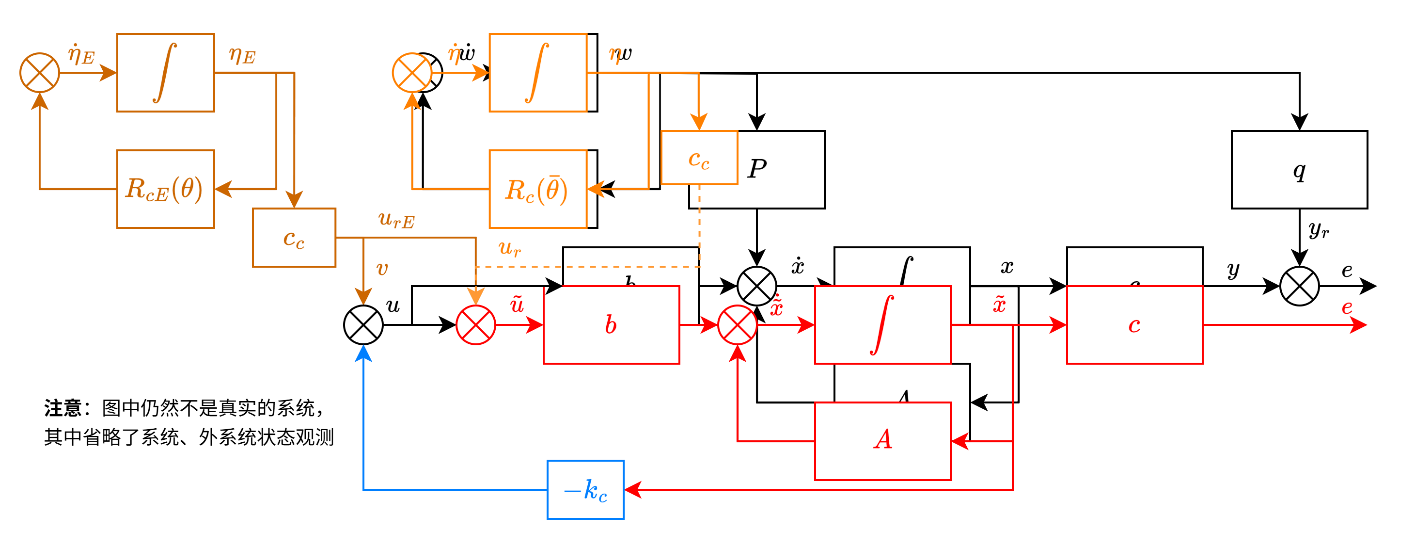
\includegraphics[width=6.42609in,height=2.48484in]{media/image5.png} \\
\end{longtable}

*如果状态空间模型由传递函数模型得到（使用标准型表示），称之为实现问题。

*实现问题是指由系统的传递函数矩阵/脉冲响应函数矩阵来建立\textbf{与其在输入输出特性上等价的状态空间}（传递函数矩阵的实现/脉冲响应函数矩阵的实现）的过程。

*SISO系统的状态空间实现能控、能观 ↔
传递函数模型零极点对消，这和Landau等人的研究是一致的。

\subsection{参数化估计内模与状态观测、实际耦合系统}\label{ux53c2ux6570ux5316ux4f30ux8ba1ux5185ux6a21ux4e0eux72b6ux6001ux89c2ux6d4bux5b9eux9645ux8026ux5408ux7cfbux7edf}

假设系统状态\(\widetilde{x}\)与理想内模\(\eta\)可以直接测得，那么问题就解决了，只要令\(u = k_{c}\widetilde{x} + c_{c}\eta\)即可。然而这两部分均不可直接得到，为此需要分别解决\textbf{系统状态不可测}、\textbf{理想内模不可测}的问题。

\begin{itemize}
\item
  构造一个自适应内模，通过获取\(\eta_{E}\)来间接设计\(v = u_{rE} = c_{c}\eta_{E}\)。由此，对于未知阶次的内模，只需给定\(m\)随后在线自适应参数\(\theta\)，此时残差\(\epsilon\)显式表示。
\item
  状态实际上不可测，因此理想控制器\(u = k_{c}\widetilde{x} + c_{c}\eta\)中的状态\({\widetilde{x}}_{o}\)需要用可观测量\({\widehat{\widetilde{x}}}_{o}\)代替。
\end{itemize}

\begin{longtable}[]{@{}
  >{\raggedright\arraybackslash}p{(\linewidth - 2\tabcolsep) * \real{0.5000}}
  >{\raggedright\arraybackslash}p{(\linewidth - 2\tabcolsep) * \real{0.5000}}@{}}
\toprule\noalign{}
\multicolumn{2}{@{}>{\raggedright\arraybackslash}p{(\linewidth - 2\tabcolsep) * \real{1.0000} + 2\tabcolsep}@{}}{%
\begin{minipage}[b]{\linewidth}\raggedright
\textbf{参数化估计内模}

真实参数化内模

\[\begin{aligned}
\dot{\eta} = & R_{c}\left( \overline{\theta} \right)\eta,\ \ \eta(0) = \eta_{0},\ \ \eta \in \mathbf{R}^{2r + 1} \\
u_{r} = & c_{c}\eta
\end{aligned}\]

由于不知道``真实内模''的阶次\(r\)，我们可以先设想一个阶次\(m\)的内模

\[\begin{aligned}
{\dot{\eta}}_{E} = & R_{cE}(\theta)\eta_{E},\ \ \eta_{E}(0) = \eta_{E0},\ \ \eta_{E} \in \mathbf{R}^{2m + 1} \\
u_{rE} = & c_{c}\eta_{E}
\end{aligned}\]

其中\(\overline{\theta} = \left\lbrack {\overline{\theta}}_{1},\ \ldots,\ {\overline{\theta}}_{r} \right\rbrack^{\top}\)，\(\theta = \left\lbrack \theta_{1},\ \ldots,\theta_{m} \right\rbrack^{\top}\)。

其中\(R_{cE}(\theta) = A_{c} - \sum_{i = 1}^{m}\theta_{i}E_{2i}\eta_{E1} = {\begin{bmatrix}
0 & 1 & & & & & \\
 - \theta_{1} & 0 & 1 & & & & \\
0 & 0 & & 1 & & & \\
 - \theta_{2} & 0 & & & 1 & & \\
 \vdots & \vdots & & & & \ddots & \\
{- \theta}_{m} & 0 & & & & & 1 \\
0 & 0 & & & & & 0
\end{bmatrix}}_{(2m + 1) \times (2m + 1)}\)
\end{minipage}} \\
\midrule\noalign{}
\endhead
\bottomrule\noalign{}
\endlastfoot
\textbf{（1）}\(\mathbf{m}\mathbf{< r}\) \textbf{欠参数化}

设\(S = \{\theta_{E} \mid s^{2m} + \theta_{E1}s^{2m - 1} + \ldots + \theta_{Em} = 0,\ s \subset \{ \pm j\omega_{1},\ \ldots, \pm j\omega_{r}\}\} \subset \mathbf{R}^{m}\)

为所有可能向量\(\theta_{E} = \left\lbrack \theta_{E1},\ldots,\theta_{Em} \right\rbrack^{\top}\)的集合

当\(\theta = \theta_{E}\)且初始条件设为\(\eta_{E}(0)\)时

\(\epsilon_{M}(m) = \min_{\substack{\theta_{E} \in S \\ \eta_{E0} \in R^{2m + 1}}}{\sup_{t \geq 0}\left| u_{r}(t) - u_{rE}\left( t,\theta_{E},\eta_{E}(0) \right) \right|}\)
& \textbf{（2）}\(\mathbf{m \geq r}\) \textbf{过参数化}

\(\theta = \left\lbrack {\overline{\theta}}^{\top},0,\ldots,0 \right\rbrack^{\top},\eta_{E0} = \left\lbrack \eta_{0}^{\top},\ 0,\ \ldots,\ 0 \right\rbrack^{\top}\)

最小值

\(\epsilon_{M}(m) = 0\) \\
\multicolumn{2}{@{}>{\raggedright\arraybackslash}p{(\linewidth - 2\tabcolsep) * \real{1.0000} + 2\tabcolsep}@{}}{%
\textbf{状态反馈与状态观测}

被控系统\((A,b)\)能控保证了存在状态反馈\(u = k_{c}{\widetilde{x}}_{o} + v\)保证\((A_{o} + b_{o}k_{c})\)Hurwitz，其中待设计信号\(v\)专门补偿未知的\(u_{r}\)；需要注意的是，在这里，反馈控制需要基于状态观测器，实际上

\(u = k_{c}{\widehat{\widetilde{x}}}_{o} + v\)

状态观测器构建如下：

\({\dot{\widehat{\widetilde{x}}}}_{o} = A_{o}\widehat{\widetilde{x}} + b_{o}k_{c}{\widehat{\widetilde{x}}}_{o} - k_{o}(e - c_{o}{\widehat{\widetilde{x}}}_{o})\)

可以证明，若能保证信号\(v(t)\)有界，则\({\widetilde{e}}_{o} = {\widetilde{x}}_{o} - {\widehat{\widetilde{x}}}_{o}\)，\({\widetilde{x}}_{o}\)均为有界的。} \\
\multicolumn{2}{@{}>{\raggedright\arraybackslash}p{(\linewidth - 2\tabcolsep) * \real{1.0000} + 2\tabcolsep}@{}}{%
\textbf{能观系统}

考虑到外系统建模偏差/未建模动态的存在：\(\epsilon(t) = u_{r}(t) - u_{rE}(t)\)，可以重新构想能观系统：

\(\begin{aligned}
\begin{bmatrix}
{\dot{\widehat{\widetilde{x}}}}_{o} \\
{\dot{\eta}}_{E}
\end{bmatrix} = & \begin{bmatrix}
A_{o} & - b_{o}c_{c} \\
0 & R_{cE}(\theta)
\end{bmatrix}\begin{bmatrix}
{\widehat{\widetilde{x}}}_{o} \\
\eta_{E}
\end{bmatrix} + \begin{bmatrix}
b_{o} \\
0
\end{bmatrix}(u - \epsilon),\ \ {\widehat{\widetilde{x}}}_{o} \in \mathbf{R}^{v},\eta_{E} \in \mathbf{R}^{2m + 1},u,\epsilon \in \mathbf{R} \\
e = & {\begin{bmatrix}
c_{o} & 0
\end{bmatrix}\begin{bmatrix}
{\widehat{\widetilde{x}}}_{o} \\
\eta_{E}
\end{bmatrix},\ \ y}_{r} = - qw,\ \ y = cx,\ \ y,y_{r},e \in \mathbf{R}
\end{aligned}\)} \\
\end{longtable}

此时内模虽然可测，却带来了新的问题。

\begin{enumerate}
\def\labelenumi{\arabic{enumi}.}
\item
  引入了显式的估计偏差\(\epsilon(t)\)；
\item
  需要为参数\(\theta\)设计合理的参数自适应算法。
\end{enumerate}

在当前系统中这两个问题无法得到很好的解决，为此Marino和Tomei提出了下面的变换设计。

\subsection{观测器标准型、滤波变换、参数自适应分析}\label{ux89c2ux6d4bux5668ux6807ux51c6ux578bux6ee4ux6ce2ux53d8ux6362ux53c2ux6570ux81eaux9002ux5e94ux5206ux6790}

文中的滤波变换（filtered
transformation）是Marino和Tomei早期在自适应观测器设计中提出的一种核心技巧，其思想是，通过线性滤波器对原始系统信号进行动态扩展，\textbf{使未知系数以``线性回归''形式出现}，从而简化参数估计与收敛分析。

\begin{enumerate}
\def\labelenumi{\arabic{enumi}.}
\item
  \textbf{把非线性或耦合项转化为``线性回归模型''}，让参数估计器可以使用简单的梯度/投影算法；
\item
  \textbf{通过设计滤波器多项式}\(d(s)\)，人为提高系统的相对阶次，获得一个严格正实（SPR）的结构，从而在稳定性分析中构造合适的Lyapunov函数。
\end{enumerate}

\subsubsection{线性坐标变换}\label{ux7ebfux6027ux5750ux6807ux53d8ux6362}

\begin{longtable}[]{@{}
  >{\raggedright\arraybackslash}p{(\linewidth - 0\tabcolsep) * \real{1.0000}}@{}}
\toprule\noalign{}
\begin{minipage}[b]{\linewidth}\raggedright
\textbf{观测器标准型 坐标变换（change of coordinates）}

由于上述增广系统能观，存在坐标变换\(\zeta = T_{2}(\theta)\begin{bmatrix}
{\widehat{\widetilde{x}}}_{o} \\
\eta_{E}
\end{bmatrix}\)，\(\zeta \in \mathbf{R}^{v + 2m + 1}\)，变换后的系统变为\textbf{观测器标准型（observer
canonical form）}：

\[\begin{aligned}
\dot{\zeta} = & A_{c}\zeta + \left\{ - a\lbrack 0\rbrack e + b\lbrack 0\rbrack(u - \epsilon) \right\} + \sum_{i = 1}^{m}\theta_{i}\left\{ - a\lbrack i\rbrack e + b\lbrack i\rbrack(u - \epsilon) \right\} \\
e = & c_{c}\zeta
\end{aligned}\]
\end{minipage} \\
\midrule\noalign{}
\endhead
\bottomrule\noalign{}
\endlastfoot
\end{longtable}

\subsubsection{滤波变换}\label{ux6ee4ux6ce2ux53d8ux6362}

\begin{longtable}[]{@{}
  >{\raggedright\arraybackslash}p{(\linewidth - 0\tabcolsep) * \real{1.0000}}@{}}
\toprule\noalign{}
\begin{minipage}[b]{\linewidth}\raggedright
\textbf{滤波变换（filtered transformation）}

\[z = \zeta - \begin{bmatrix}
0 \\
\sum_{i = 1}^{m}{\xi_{i}\theta_{i}}
\end{bmatrix},\ z \in \mathbf{R}^{v + 2m + 1}\]

其中\({\dot{\xi}}_{i} = D\xi_{i} + \begin{bmatrix}
0 & I_{v + 2m}
\end{bmatrix}\left( - a\lbrack i\rbrack e + b\lbrack i\rbrack u \right),\ \ \xi_{i}(0) = \xi_{i0} \in \mathbf{R}^{v + 2m}\)

\[\dot{z} + \begin{bmatrix}
0 \\
\sum_{i = 1}^{m}{\xi_{i}\theta_{i}}
\end{bmatrix}^{'} = A_{c}\left\{ z + \begin{bmatrix}
0 \\
\sum_{i = 1}^{m}{\xi_{i}\theta_{i}}
\end{bmatrix} \right\} + \left\{ - a\lbrack 0\rbrack e + b\lbrack 0\rbrack(u - \epsilon) \right\} + \sum_{i = 1}^{m}\theta_{i}\left\{ - a\lbrack i\rbrack e + b\lbrack i\rbrack(u - \epsilon) \right\}\]

\[\begin{aligned}
\dot{z} = & A_{c}z + \sum_{i = 1}^{m}\theta_{i}\left\{ A_{c}\begin{bmatrix}
0 \\
\xi_{i}
\end{bmatrix} - \begin{bmatrix}
0 \\
{\dot{\xi}}_{i}
\end{bmatrix} \right\} + \left\{ - a\lbrack 0\rbrack e + b\lbrack 0\rbrack(u - \epsilon) \right\} + \sum_{i = 1}^{m}\theta_{i}\left\{ - a\lbrack i\rbrack e + b\lbrack i\rbrack(u - \epsilon) \right\} \\
 = & A_{c}z + \sum_{i = 1}^{m}\theta_{i}\left\{ A_{c}\begin{bmatrix}
0 \\
\xi_{i}
\end{bmatrix} - \begin{bmatrix}
0 & 0 \\
0 & D
\end{bmatrix}\begin{bmatrix}
0 \\
\xi_{i}
\end{bmatrix} - \begin{bmatrix}
0 & 0 \\
0 & I_{v + 2m}
\end{bmatrix}\left( - a\lbrack i\rbrack e + b\lbrack i\rbrack u \right) \right\} + \left\{ - a\lbrack 0\rbrack e + b\lbrack 0\rbrack u \right\} \\
 & + \sum_{i = 1}^{m}\theta_{i}\left\{ - a\lbrack i\rbrack e + b\lbrack i\rbrack u \right\} - \left( b\lbrack 0\rbrack + \sum_{i = 1}^{m}\theta_{i}b\lbrack i\rbrack \right)\epsilon \\
\dot{z} = & A_{c}z + \left\{ - a\lbrack 0\rbrack e + b\lbrack 0\rbrack u \right\} + d\sum_{i = 1}^{m}{\mu_{i}\theta_{i}} - \left( b\lbrack 0\rbrack + \sum_{i = 1}^{m}\theta_{i}b\lbrack i\rbrack \right)\epsilon \\
e = & c_{c}z
\end{aligned}\]

*滤波变换将非线性控制问题转化为可借助线性滤波技术进行状态估计和参数辨识的形式。

*多级滤波级联将输入信号转换为了多个带指数衰减的记忆分量，而坐标变换则是对系统原状态进行了滤波的修正（通过扣除经过滤波的输入分量），最终隔离出未知参数项。这个过程与系统辨识中，``把输入输出通过已知滤波器处理以构造回归向量''十分相似。
\end{minipage} \\
\midrule\noalign{}
\endhead
\bottomrule\noalign{}
\endlastfoot
\end{longtable}

\subsubsection{参数自适应收敛性分析}\label{ux53c2ux6570ux81eaux9002ux5e94ux6536ux655bux6027ux5206ux6790}

\begin{longtable}[]{@{}
  >{\raggedright\arraybackslash}p{(\linewidth - 0\tabcolsep) * \real{1.0000}}@{}}
\toprule\noalign{}
\begin{minipage}[b]{\linewidth}\raggedright
\textbf{参数自适应算法}

通过滤波变换，可以完成自适应观测器的设计（\(i = 1,\ldots,m\)）：

\[\begin{aligned}
\dot{\widehat{z}} = & A_{c}\widehat{z} + \left\{ - a\lbrack 0\rbrack e + b\lbrack 0\rbrack u \right\} + d\sum_{i = 1}^{m}{\mu_{i}{\widehat{\theta}}_{i}} - {\overline{k}}_{o}(e - c_{c}\widehat{z}) \\
 = & A_{c}\widehat{z} + \left\{ - a\lbrack 0\rbrack e + b\lbrack 0\rbrack u \right\} + d\sum_{i = 1}^{m}{\mu_{i}{\widehat{\theta}}_{i}} - {\overline{k}}_{o}c_{c}\widetilde{z} \\
e = & c_{c}z
\end{aligned}\]

其中观测器增益选择为\({\overline{k}}_{o} = - \left( A_{c} + \lambda I \right)d\)，这一选择能够保证\((A_{c} + {\overline{k}}_{o}c_{c},d,c_{c})\)严格正实（SPR）。

可为上述系统设计参数自适应算法：

\[{\dot{\widehat{\theta}}}_{\mathbf{i}}\mathbf{=}\left\{ \begin{aligned}
\mathbf{\&}{g_{i}\mu}_{i}\left( e - c_{c}\widehat{z} \right) & 0 \leq t \leq T_{M} \\
\mathbf{\&}\left\{ \begin{array}{rlrlr}
 & g_{i}\mu_{i}\left( e - c_{c}\widehat{z} \right) & & & \det\left\lbrack M_{i}(t) \right\rbrack \geq m_{0}e^{- \lambda_{0}t} > 0 \\
 & g_{i}\mu_{i}\left( e - c_{c}\widehat{z} \right) - \alpha_{i}{\widehat{\theta}}_{i} & & & otherwise
\end{array} \right.\  & t > T_{M}
\end{aligned} \right.\ \]

其中\(M_{i}(t) = \int_{t - T_{M}}^{t}{\mu\lbrack i\rbrack(\tau)\mu\lbrack i\rbrack(\tau)^{\top}}d\tau\)
\end{minipage} \\
\midrule\noalign{}
\endhead
\bottomrule\noalign{}
\endlastfoot
\end{longtable}

\textbf{持续激励条件（persistently
exciting）与外部扰动}\(\mathbf{u}_{\mathbf{r}}\left( \mathbf{t} \right)\)\textbf{的频率内容直接相关}：由Sastry
and
Bodson,1989可证明，如果扰动\(\mathbf{u}_{\mathbf{r}}\left( \mathbf{t} \right)\)\textbf{包含}\(\mathbf{i}^{\mathbf{*}}\)\textbf{个不同的正弦频率分量}，那么由滤波器生成的\textbf{回归信号向量}\(\mathbf{\mu}\left\lbrack \mathbf{i}^{\mathbf{*}} \right\rbrack\left( \mathbf{t} \right)\mathbf{=}\left\lbrack \mathbf{\mu}_{\mathbf{1}}\left( \mathbf{t} \right)\mathbf{,\ldots,\ }\mathbf{\mu}_{\mathbf{i}^{\mathbf{*}}}\left( \mathbf{t} \right) \right\rbrack^{\mathbf{\top}}\)\textbf{也会是持续激励的}，此时\(M_{i}(t)\)在有限时间窗\(T_{M}\)内保持非奇异。简单说，扰动中有多少个不同的频率，滤波器就能生成相应维度的激励信号。

\begin{itemize}
\item
  当\(m < r\)时，内模阶数不够，只能近似部分频率，存在逼近误差 ϵ(t)；
\item
  当\(m = r\)时，实际干扰维度能够覆盖内模阶数，参数收敛能够保证频率识别准确；
\item
  当\(m > r\)时，部分\(\mu_{i}\)不再有足够频率激励，对这一问题，文中通过泄漏项处理。
\end{itemize}

\begin{longtable}[]{@{}
  >{\raggedright\arraybackslash}p{(\linewidth - 0\tabcolsep) * \real{1.0000}}@{}}
\toprule\noalign{}
\begin{minipage}[b]{\linewidth}\raggedright
\textbf{{[}定理{]}信号有界性}

在4.1节介绍的（H1）\textasciitilde（H4）的假设下，自适应输出误差反馈控制器能够保证闭环系统误差\(\widetilde{\theta},z - \widehat{z},x - x_{r},e,{\widetilde{x}}_{o} - {\widehat{\widetilde{x}}}_{o}\)有界。
\end{minipage} \\
\midrule\noalign{}
\endhead
\bottomrule\noalign{}
\endlastfoot
\textbf{{[}定理{]}信号收敛性}

若近似误差\(\epsilon_{M}\)足够小，使得线性变换矩阵\(T_{2}\left( \widehat{\theta} \right)\)没有奇点，则随着\(t \rightarrow \infty\)上述闭环系统误差收敛到远点附近的一个小球内。

\textbf{欠建模（}\(\mathbf{m < r}\)\textbf{）}：只能把误差压倒\(\epsilon_{M}\)的邻域，存在不可消除残差，上限由构造的量给出。

\textbf{过建模（}\(\mathbf{m \geq r}\)\textbf{）}：\(\epsilon_{M} = 0\)，在充分的激励下能够实现\(e(t) \rightarrow 0\)。 \\
\begin{minipage}[t]{\linewidth}\raggedright
证明过程：

\begin{enumerate}
\def\labelenumi{\arabic{enumi}.}
\item
  根据观测器误差动态模型，证明滤波器输出（回归向量\(\mu_{i}\)）有界
\end{enumerate}

\[\begin{aligned}
\dot{\widetilde{z}} = & \left( A_{c} + {\overline{k}}_{o}c_{c} \right)\widetilde{z} + d\mu^{\top}\widetilde{\theta} - \epsilon\left( b\lbrack 0\rbrack + \sum_{i = 1}^{m}\theta_{i}b\lbrack i\rbrack \right) \\
{\dot{\chi}}_{i} = & D\chi_{i} + \begin{bmatrix}
0 & I_{v + 2m}
\end{bmatrix}b\lbrack i\rbrack u_{r} \\
\mu_{i} = & \begin{bmatrix}
1 & 0 & \cdots & 0
\end{bmatrix}\chi_{i}
\end{aligned}\]

\begin{quote}
只需要\(u_{r}(t)\)包含\(i^{*}\)个不同的频率成分即可保证滤波器构造的\(i^{*}\)元回归向量\(\mu\lbrack i^{*}\rbrack\)持续激励；

而干扰成分假设保证\(u_{r}(t)\)含\(r\)个频率成分，对于含\({i^{*} = \min}{\{ m,r\}}\)（欠建模情况取\(m\)，过建模情况只取\(r\)）个分量的回归向量，\(\exists k_{T} > 0,s.t.\)

\[\int_{t}^{t + T_{M}}{\mu\left\lbrack i^{*} \right\rbrack(\tau)\mu\left\lbrack i^{*} \right\rbrack^{\top}(\tau)}d\tau \geq k_{T}I > 0,\ \ \forall t \geq 0\]
\end{quote}

\begin{enumerate}
\def\labelenumi{\arabic{enumi}.}
\setcounter{enumi}{1}
\item
  欠建模（\(m \leq r\)）情况讨论
\end{enumerate}

\begin{quote}
\[{\dot{\widetilde{\theta}}}_{i} = - g_{i}\mu_{i}\left( e - c_{c}\widehat{z} \right),\ \ t \geq 0,1 \leq i \leq m\]

由于不是所有频率都得到跟踪，此时每个通道都能匹配到干扰频率，它们都会收敛
\end{quote}

\begin{enumerate}
\def\labelenumi{\arabic{enumi}.}
\setcounter{enumi}{2}
\item
  过建模（\(m > r\)）情况讨论
\end{enumerate}

\begin{quote}
\[{\dot{\widetilde{\theta}}}_{i} = - g_{i}\mu_{i}\left( e - c_{c}\widehat{z} \right),\ \ t \geq 0,1 \leq i \leq r\]

对于能够匹配干扰频率的通道，更新律仍然能够收敛

\[{\dot{\widetilde{\theta}}}_{i} = - g_{i}\mu_{i}\left( e - c_{c}\widehat{z} \right),\ \ t \geq 0,r < i \leq m\]

此时存在冗余通道，部分通道无法再匹配到干扰频率，可能发散，为此需要根据时间分区来决定是否引入泄漏项，更新律改进为：

\[{\dot{\widetilde{\theta}}}_{i} = \left\{ \begin{array}{rlr}
 & - g_{i}\mu_{i}\left( e - c_{c}\widehat{z} \right) & t \in S_{1i} \\
 & - g_{i}\mu_{i}\left( e - c_{c}\widehat{z} \right) - \alpha_{i}{\widetilde{\theta}}_{i} & t \in S_{2i}
\end{array} \right.\ ,\ \ t \geq 0,r < i \leq m\]

\(S_{1i} = \{ t \mid \det\left\lbrack M_{i}(t) \right\rbrack \geq m_{0}e^{- \lambda_{0}t},0 \leq t \leq T_{M}\}\)，在此区间内，矩阵\(M_{i}(t)\)的行列式还比较大，滤波器初始条件导致的过渡态还未衰减，暂时不引入泄漏项；

\(S_{2i} = \{ t \mid \det\left\lbrack M_{i}(t) \right\rbrack < m_{0}e^{- \lambda_{0}t}\}\)，前\(r\)通道收敛，这些通道就再也不会得到持久激励（因此\(S_{2i}\)最终会延伸到无穷）应当增加泄漏项，保证冗余参数渐近收敛到0。

总结来说，就是利用\(\mu_{i}\)是否满足持续激励来判定是否进行参数更新。
\end{quote}
\end{minipage} \\
\end{longtable}

\subsubsection{Lyapunov函数构造与收敛性分析}\label{lyapunovux51fdux6570ux6784ux9020ux4e0eux6536ux655bux6027ux5206ux6790}

观测器误差动态：\(\dot{\widetilde{z}} = \left( A_{c} + {\overline{k}}_{o}c_{c} \right)\widetilde{z} + d\mu^{\top}\widetilde{\theta} - \epsilon\left( b\lbrack 0\rbrack + \sum_{i = 1}^{m}\theta_{i}b\lbrack i\rbrack \right)\)

自适应律：\({\dot{\widetilde{\theta}}}_{i} = - g_{i}\mu_{i}\left( e - c_{c}\widehat{z} \right) = - g_{i}\mu_{i}c_{c}\widetilde{z}\)，（\(e - c_{c}\widehat{z} = c_{c}\left( z - \widehat{z} \right) = c_{c}\widetilde{z}\)）

矩阵微分方程：\({\dot{Q}}_{2} = - Q_{2} + \mu\left\lbrack i^{*} \right\rbrack\mu^{\top}\left\lbrack i^{*} \right\rbrack,\ \ Q_{2}(0) = e^{- T_{M}}k_{T}I\)

\begin{longtable}[]{@{}
  >{\raggedright\arraybackslash}p{(\linewidth - 0\tabcolsep) * \real{1.0000}}@{}}
\toprule\noalign{}
\begin{minipage}[b]{\linewidth}\raggedright
构造Lyapunov函数

\[V = {\widetilde{z}}^{\top}P\widetilde{z} + {\widetilde{\theta}}^{\top}G\widetilde{\theta} + \frac{1}{2}\beta\left( Q_{2}\widetilde{\theta}\left\lbrack i^{*} \right\rbrack - \frac{\mu\left\lbrack i^{*} \right\rbrack d^{\top}\widetilde{z}}{d^{\top}d} \right)^{\top}\left( Q_{2}\widetilde{\theta}\left\lbrack i^{*} \right\rbrack - \frac{\mu\left\lbrack i^{*} \right\rbrack d^{\top}\widetilde{z}}{d^{\top}d} \right)\]

其中第3项是为了泄漏项引入的，当\(t \in S_{i1}\)时容易证明收敛性。

矩阵\(P\)设为Lyapunov方程\(\left( A_{c} + {\overline{k}}_{o}c_{c} \right)^{\top}P + P\left( A_{c} + {\overline{k}}_{o}c_{c} \right) = - Q_{1} < 0\)的解，可证明\(Pd = c_{c}^{\top}\)，由于\((A_{c} + {\overline{k}}_{o}c_{c},d,c_{c})\)SPR，可证明方程有界；

另外，矩阵\(G\)设为\(G = diag\left\lbrack g_{1},\ldots,g_{m} \right\rbrack\)，\(G\lbrack i^{*}\rbrack = diag\left\lbrack g_{1},\ldots,g_{i^{*}} \right\rbrack\)；

向量\(\widetilde{\theta}\left\lbrack i^{*} \right\rbrack = \left\lbrack {\widetilde{\theta}}_{1},\ldots,{\widetilde{\theta}}_{i^{*}} \right\rbrack^{\top}\)，\(\mu\left\lbrack i^{*} \right\rbrack = \left\lbrack \mu_{1},\ldots,\mu_{i^{*}} \right\rbrack^{\top}\)
\end{minipage} \\
\midrule\noalign{}
\endhead
\bottomrule\noalign{}
\endlastfoot
\begin{minipage}[t]{\linewidth}\raggedright
收敛性分析

\begin{enumerate}
\def\labelenumi{\arabic{enumi}.}
\item
  过建模（\(m > r\)）情况讨论
\end{enumerate}

\[\begin{aligned}
\dot{V} = & {- \widetilde{z}}^{\top}Q_{1}\widetilde{z} + 2{\widetilde{z}}^{\top}P\left\lbrack d\mu^{\top}\widetilde{\theta} - \epsilon\left( b\lbrack 0\rbrack + \sum_{i = 1}^{m}\theta_{i}b\lbrack i\rbrack \right) \right\rbrack \\
 + & {2\widetilde{\theta}}^{\top}G\widetilde{\theta} \\
 + & \beta\left( Q_{2}\widetilde{\theta}\left\lbrack i^{*} \right\rbrack - \frac{\mu\left\lbrack i^{*} \right\rbrack d^{\top}\widetilde{z}}{d^{\top}d} \right)^{\top}\left\{ \begin{array}{r}
\left( - Q_{2} + \mu\left\lbrack i^{*} \right\rbrack\mu^{\top}\left\lbrack i^{*} \right\rbrack \right)\widetilde{\theta}\left\lbrack i^{*} \right\rbrack + Q_{2}\widetilde{\theta}\left\lbrack i^{*} \right\rbrack - \frac{\dot{\mu}\left\lbrack i^{*} \right\rbrack d^{\top}\widetilde{z}}{d^{\top}d} - \frac{\mu\left\lbrack i^{*} \right\rbrack d^{\top}}{d^{\top}d}\widetilde{z}
\end{array} \right\}
\end{aligned}\]

\begin{enumerate}
\def\labelenumi{\arabic{enumi}.}
\setcounter{enumi}{1}
\item
  欠建模（\(m \leq r\)）情况讨论
\end{enumerate}
\end{minipage} \\
\end{longtable}

\subsubsection{推导过程}\label{ux63a8ux5bfcux8fc7ux7a0b}

\begin{longtable}[]{@{}
  >{\raggedright\arraybackslash}p{(\linewidth - 0\tabcolsep) * \real{1.0000}}@{}}
\toprule\noalign{}
\begin{minipage}[b]{\linewidth}\raggedright
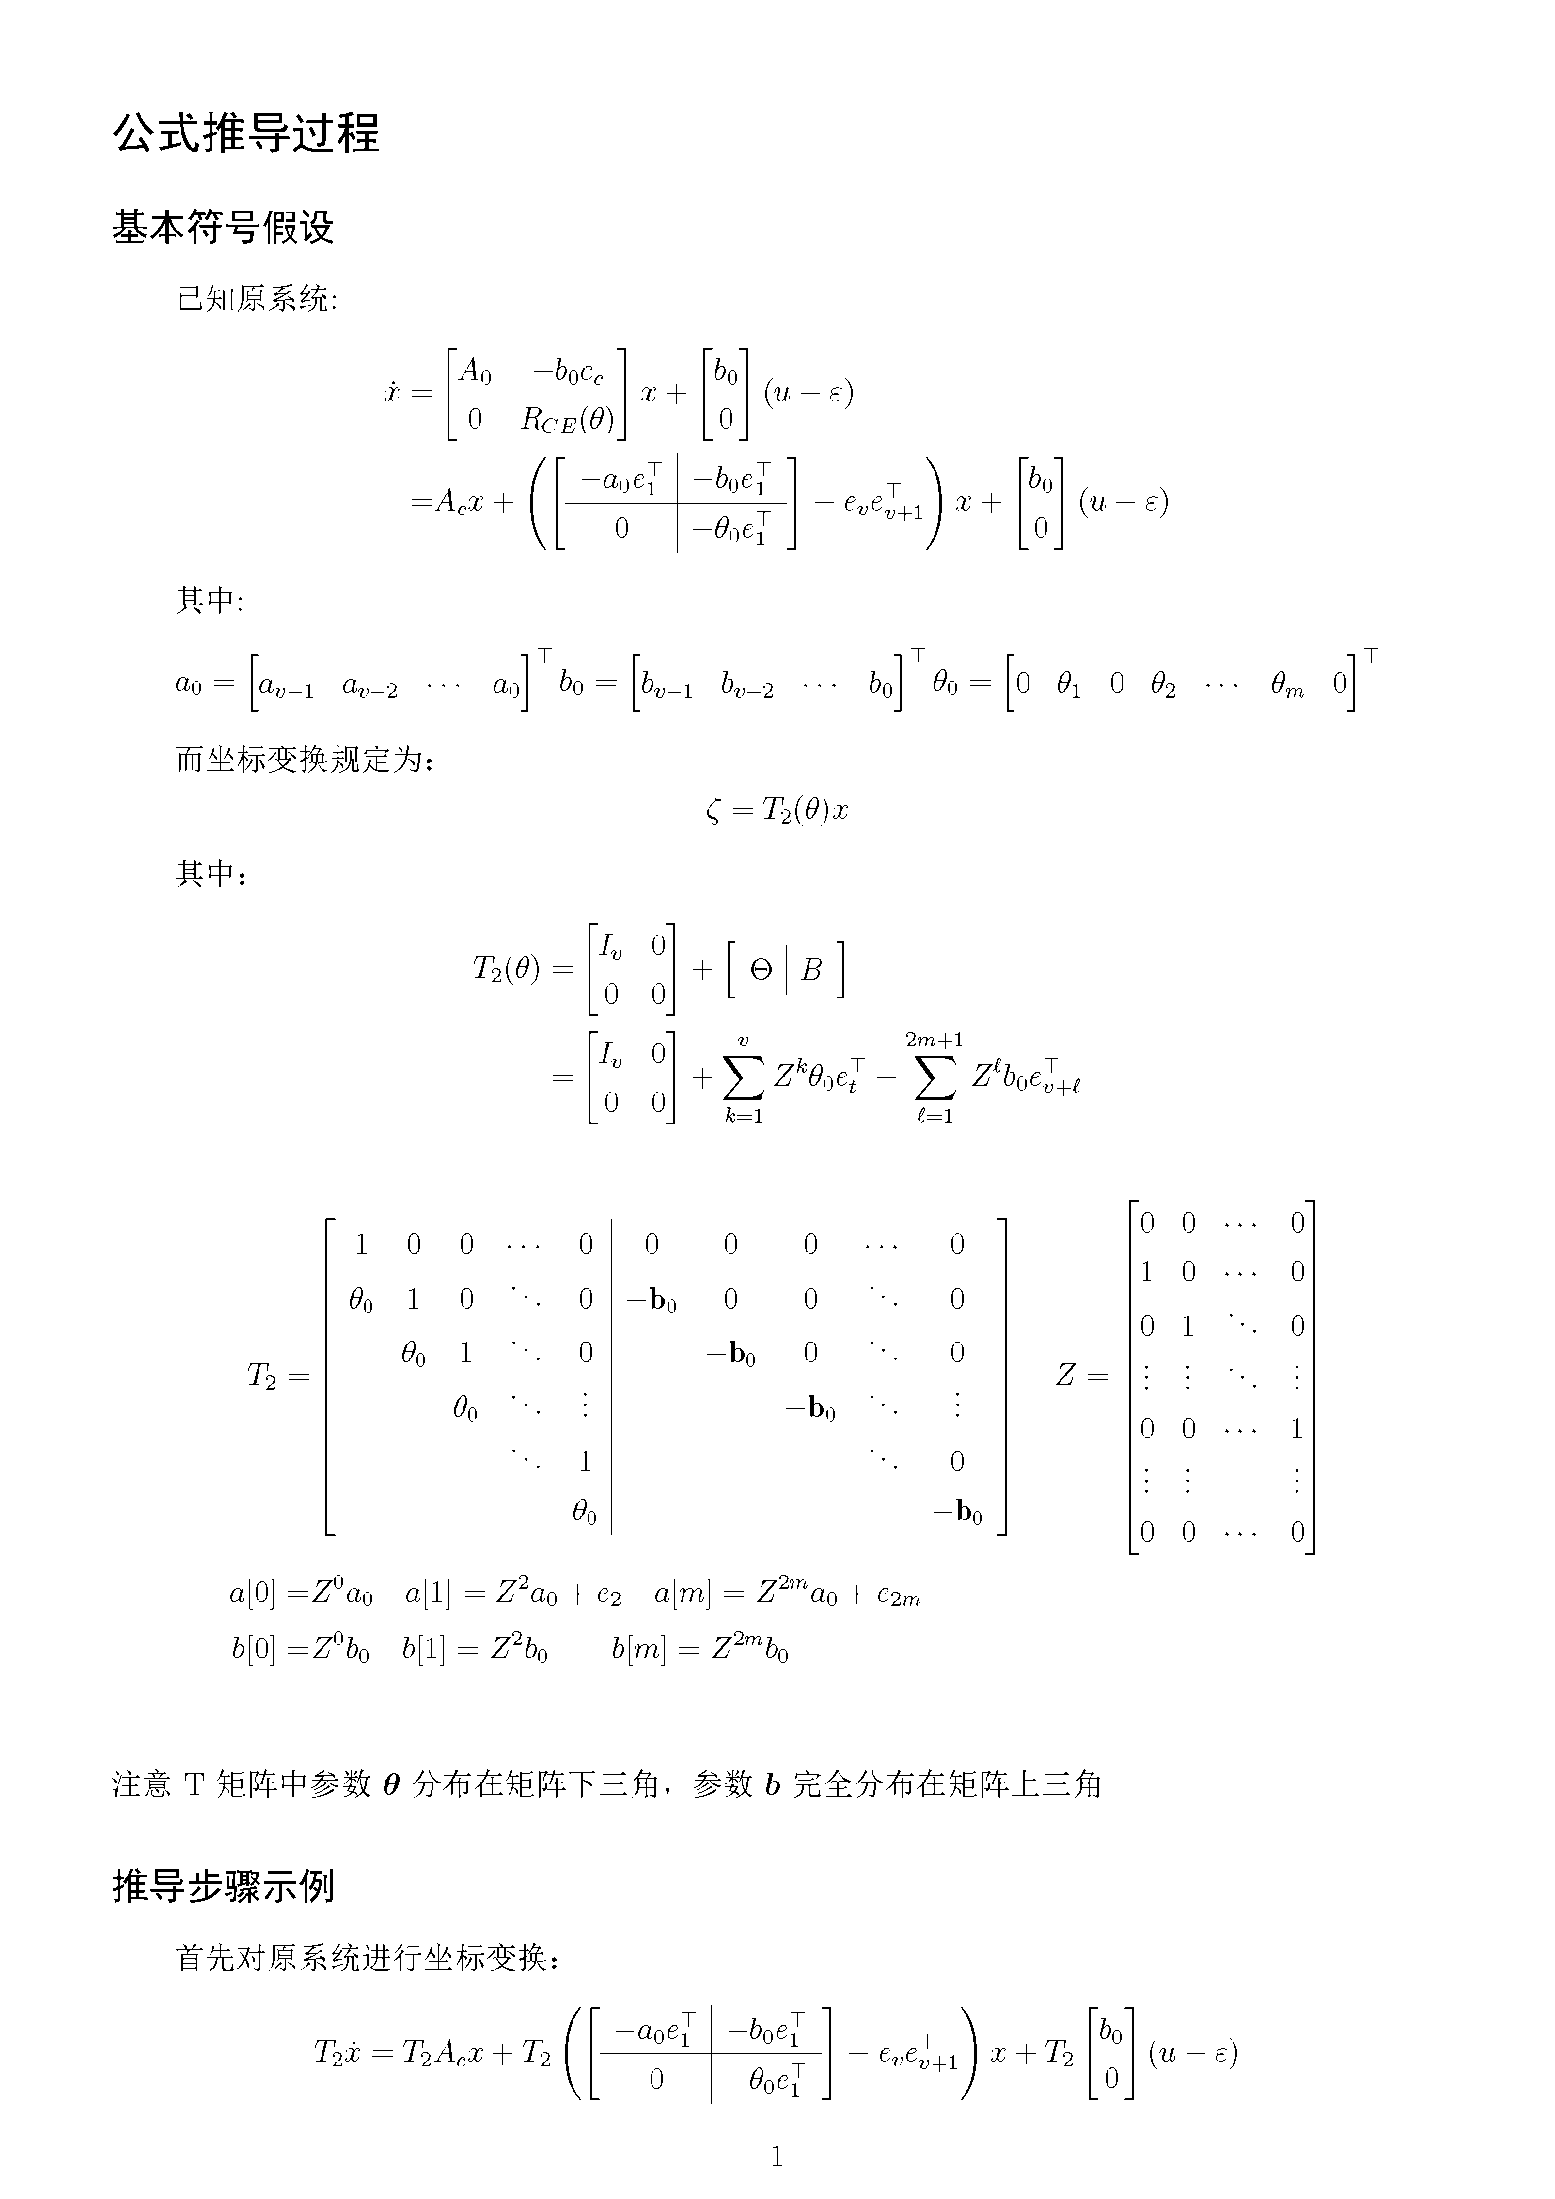
\includegraphics[width=6.83958in,height=9.67153in]{media/image6.png}
\end{minipage} \\
\midrule\noalign{}
\endhead
\bottomrule\noalign{}
\endlastfoot
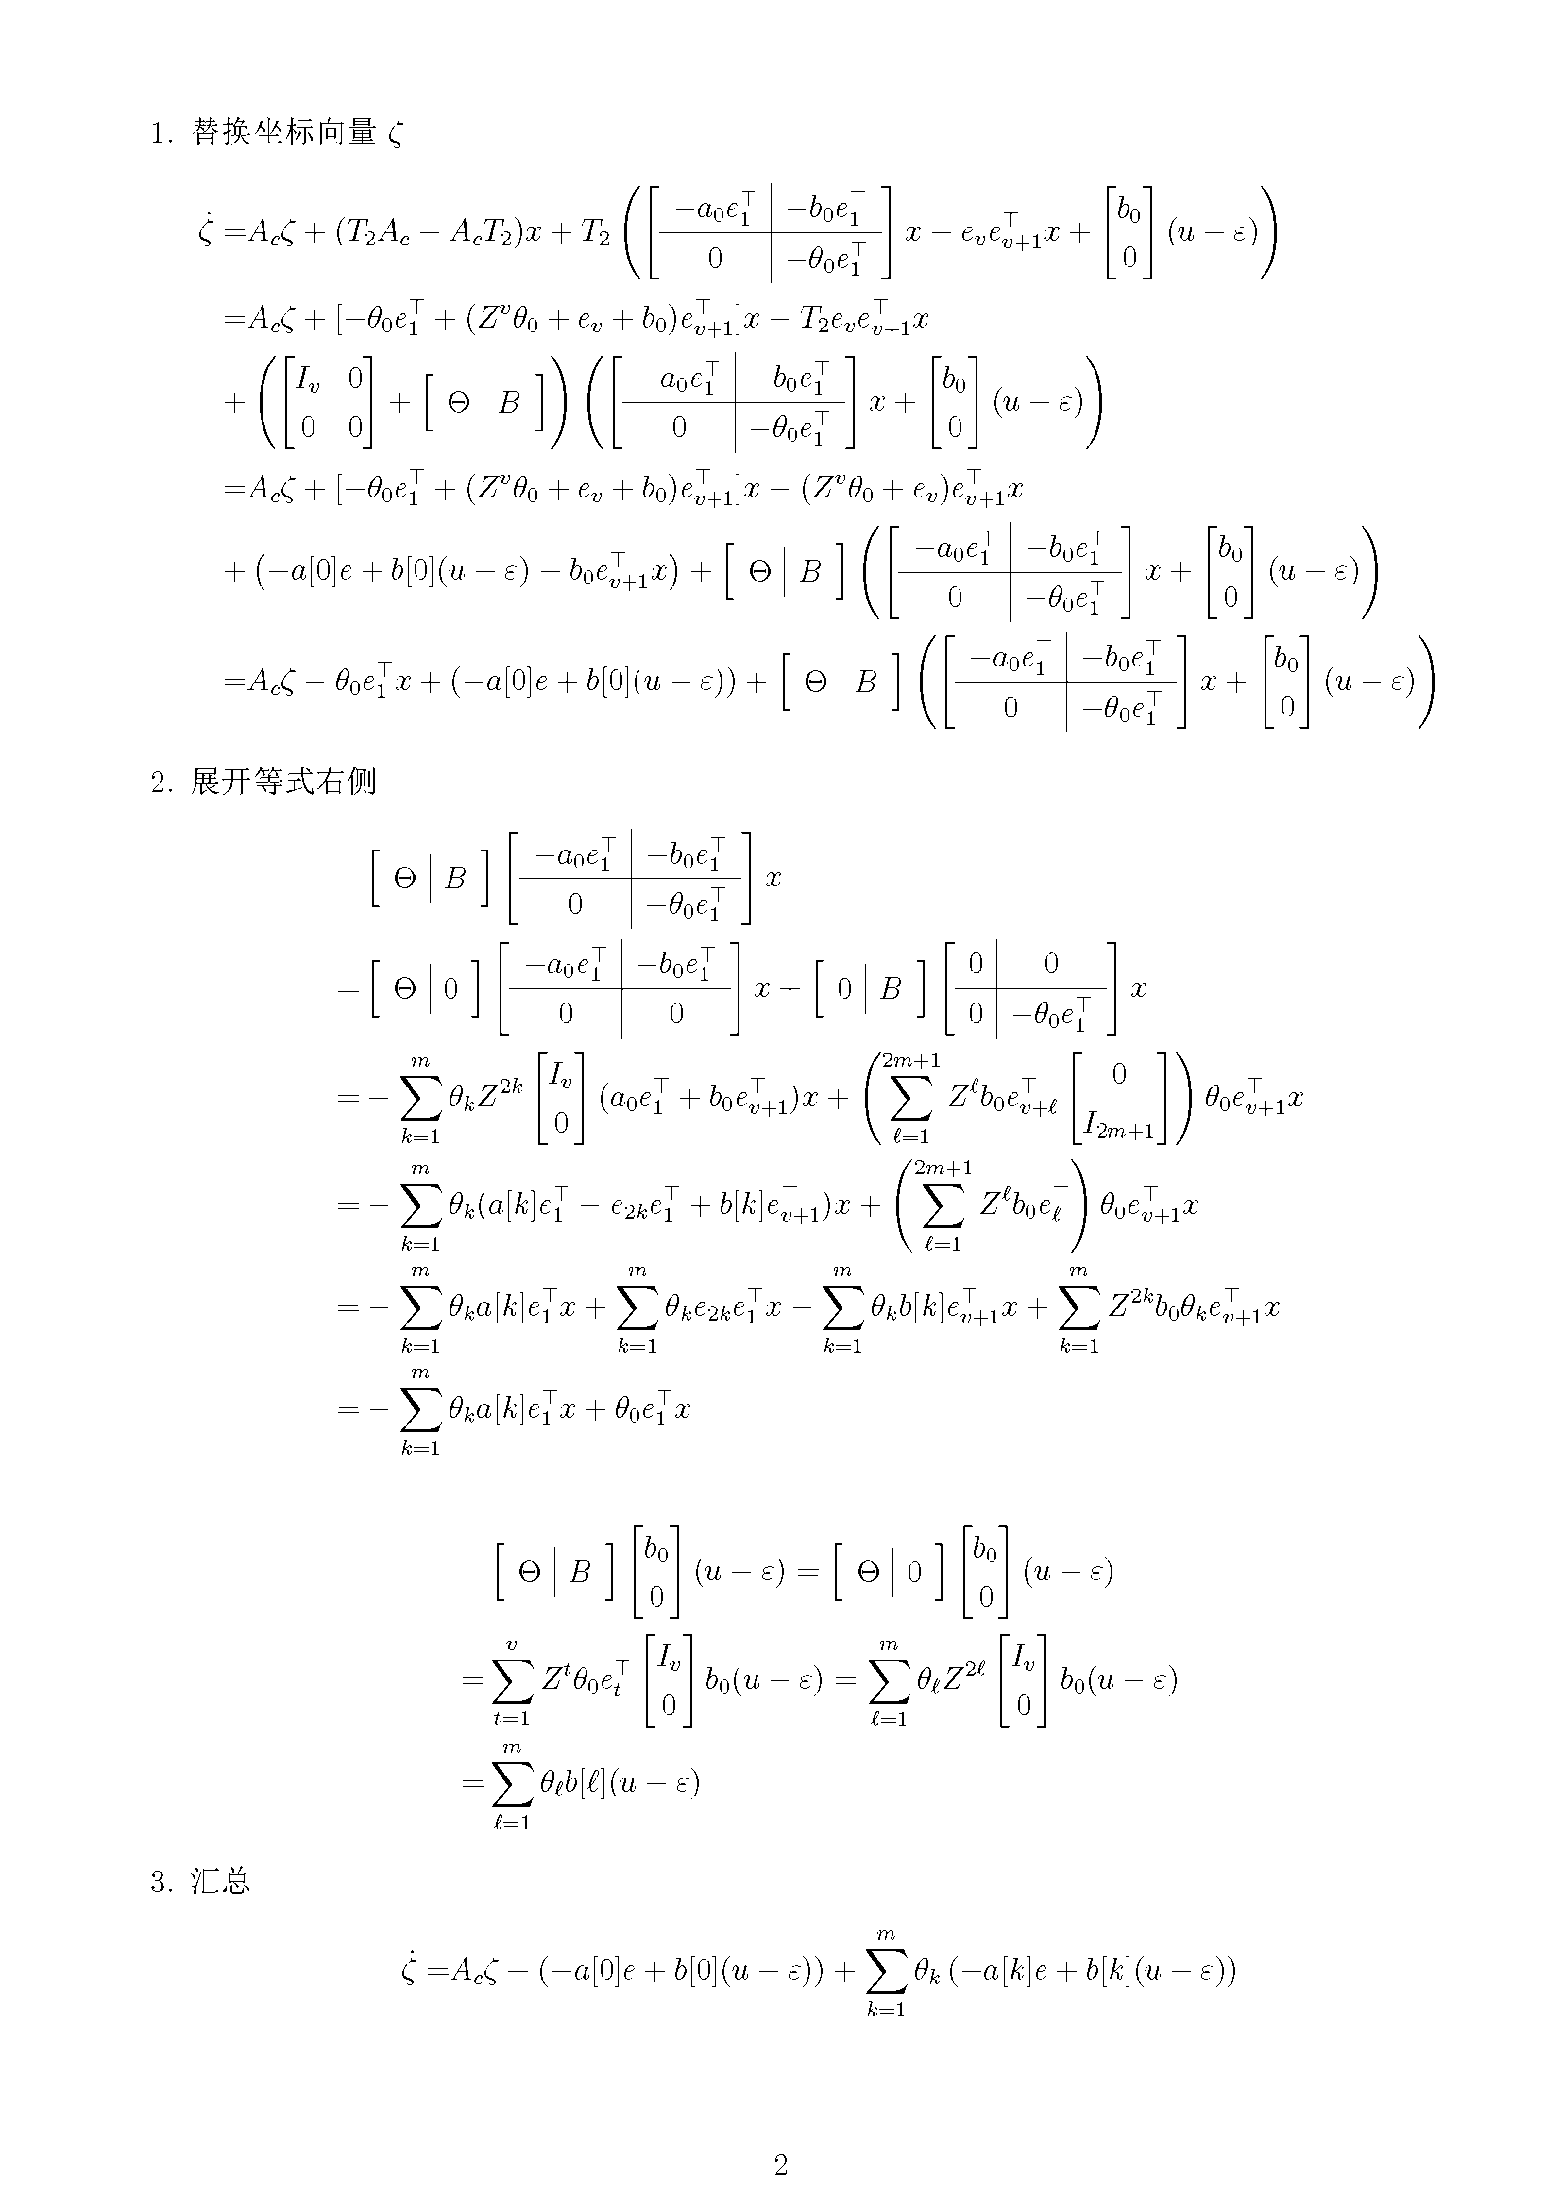
\includegraphics[width=6.98403in,height=9.87708in]{media/image7.png} \\
\end{longtable}

\subsection{完整的控制器结构}\label{ux5b8cux6574ux7684ux63a7ux5236ux5668ux7ed3ux6784}

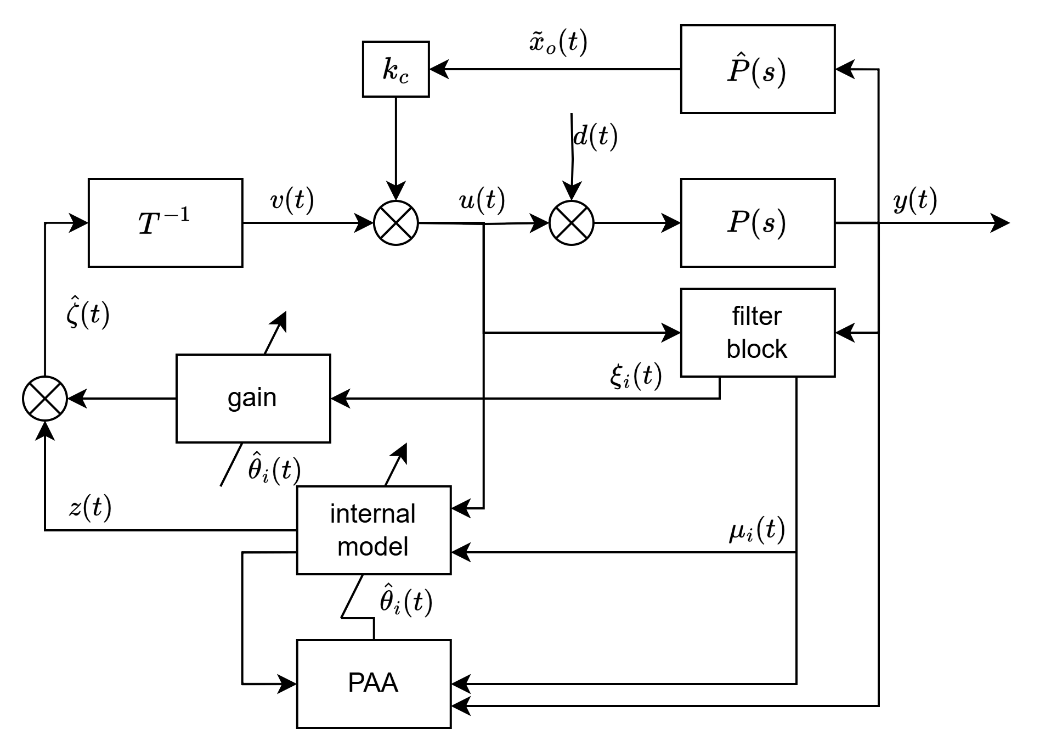
\includegraphics[width=4.46821in,height=3.19024in]{media/image8.png}

\emph{*注意图中结构仅为示意，干扰并不一定仅作用在系统输入端，外源输入同时作用在状态与输出}

控制器类似于Landau提供的控制器，它至少由三部分组成：

\begin{enumerate}
\def\labelenumi{\arabic{enumi}.}
\item
  首先是级联低通滤波器块，这一组滤波器块生成\(m\)组\(v + 2m\)维状态向量\(\xi_{i}(t)\)和观测向量\(\mu_{i}(t)\)；
\item
  参数自适应算法选用梯度算法，以观测向量为梯度方向；
\item
  自适应内模则使用观测向量、滤波器状态向量（各级滤波输出）、输入信号合成控制信号\(\widehat{\zeta}(t)\)。
\end{enumerate}

由于此控制器结构中的状态变量相对于原系统经过滤波变换，最后需要将控制信号经过逆变换得到

\[v = u_{rE} = \eta_{E1} = \left\lbrack 0,c_{c} \right\rbrack T_{2}^{- 1}\widehat{\zeta}\]

\begin{longtable}[]{@{}
  >{\raggedright\arraybackslash}p{(\linewidth - 0\tabcolsep) * \real{1.0000}}@{}}
\toprule\noalign{}
\begin{minipage}[b]{\linewidth}\raggedright
\textbf{控制器设计}

\[\begin{aligned}
u = & k_{c}{\widehat{\widetilde{x}}}_{o} + v,\ \ T_{2} \in \mathbf{R}^{n \times n},\ \ \widehat{\zeta} \in \mathbf{R}^{n} \\
v = & \left\lbrack 0_{1 \times v}\ \mid\ \begin{matrix}
1 & 0 & \cdots & 0
\end{matrix} \right\rbrack adj\left\lbrack T_{2}\left( \widehat{\theta} \right) \right\rbrack\frac{\det\left\lbrack T_{2}\left( \widehat{\theta} \right) \right\rbrack}{sat\left( {\det\left\lbrack T_{2}\left( \widehat{\theta} \right) \right\rbrack}^{2} \right)}\widehat{\zeta}
\end{aligned}\]
\end{minipage} \\
\midrule\noalign{}
\endhead
\bottomrule\noalign{}
\endlastfoot
\textbf{能观系统观测（非自适应观测器）}

\({\dot{\widehat{\widetilde{x}}}}_{o} = A_{o}{\widehat{\widetilde{x}}}_{o} + b_{o}k_{c}{\widehat{\widetilde{x}}}_{o} - k_{o}(e - c_{o}{\widehat{\widetilde{x}}}_{o})\) \\
\begin{minipage}[t]{\linewidth}\raggedright
\textbf{内模观测}

\begin{enumerate}
\def\labelenumi{\arabic{enumi}.}
\item
  \textbf{内模（自适应观测器）}
\end{enumerate}

\[\begin{aligned}
\dot{\widehat{z}} = & A_{c}\widehat{z} + ( - a\lbrack 0\rbrack e + b\lbrack 0\rbrack u) + d\sum_{i = 1}^{m}{\mu_{i}{\widehat{\theta}}_{i}} + (A_{c} + \lambda I)d\left( e - c_{c}\widehat{z} \right) \\
\widehat{\zeta} = & \widehat{z} + \begin{bmatrix}
0 \\
\sum_{i = 1}^{m}{\xi_{i}{\widehat{\theta}}_{i}}
\end{bmatrix},\ \ \widehat{z} \in \mathbf{R}^{n}
\end{aligned}\]

\begin{enumerate}
\def\labelenumi{\arabic{enumi}.}
\setcounter{enumi}{1}
\item
  \textbf{参数自适应}
\end{enumerate}

\[{\dot{\widehat{\theta}}}_{\mathbf{i}}\mathbf{=}\left\{ \begin{aligned}
\mathbf{\&}{g_{i}\mu}_{i}\left( e - c_{c}\widehat{z} \right) & 0 \leq t \leq T_{M} \\
\mathbf{\&}\left\{ \begin{array}{rlrlr}
 & g_{i}\mu_{i}\left( e - c_{c}\widehat{z} \right) & & & \det\left\lbrack M_{i}(t) \right\rbrack \geq m_{0}e^{- \lambda_{0}t} > 0 \\
 & g_{i}\mu_{i}\left( e - c_{c}\widehat{z} \right) - \alpha_{i}{\widehat{\theta}}_{i} & & & otherwise
\end{array} \right.\  & t > T_{M}
\end{aligned} \right.\ \]

\begin{enumerate}
\def\labelenumi{\arabic{enumi}.}
\setcounter{enumi}{2}
\item
  \textbf{滤波器组（滤波观测向量）}
\end{enumerate}

\[\begin{aligned}
{\dot{\xi}}_{i} = & D\xi_{i} + \begin{bmatrix}
0 & I_{v + 2m}
\end{bmatrix}\left( - a\lbrack i\rbrack e + b\lbrack i\rbrack u \right) \\
\mu_{i} = & \begin{bmatrix}
1 & 0 & \begin{matrix}
\cdots & 0
\end{matrix}
\end{bmatrix}\xi_{i},\ \ \xi_{i} \in \mathbf{R}^{n - 1}
\end{aligned}\]
\end{minipage} \\
\end{longtable}

\subsubsection{多频率信号估计}\label{ux591aux9891ux7387ux4fe1ux53f7ux4f30ux8ba1}

上面介绍了Marino与Tomei于2013年Automatica文章中介绍的控制器设计。在此之前2012年发表于Int.
J. Adapt. Control Signal
Process的未知线性外系统鲁棒自适应观测器设计从另一个角度介绍了这一问题，根据分析，鲁棒自适应观测器实际上就是前者在忽略系统模型时的特例。

\begin{longtable}[]{@{}
  >{\raggedright\arraybackslash}p{(\linewidth - 0\tabcolsep) * \real{1.0000}}@{}}
\toprule\noalign{}
\begin{minipage}[b]{\linewidth}\raggedright
\textbf{直接对应？}

\[u = v = {\widehat{\eta}}_{1} = \left\lbrack 0_{1 \times v}\ \mid\ \begin{matrix}
1 & 0 & \cdots & 0
\end{matrix} \right\rbrack adj\left\lbrack T_{2}\left( \widehat{\theta} \right) \right\rbrack\frac{\det\left\lbrack T_{2}\left( \widehat{\theta} \right) \right\rbrack}{sat\left( {\det\left\lbrack T_{2}\left( \widehat{\theta} \right) \right\rbrack}^{2} \right)}\widehat{\zeta}\]

\textbf{其中内模观测包括}：

\begin{enumerate}
\def\labelenumi{\arabic{enumi}.}
\item
  \textbf{内模}
\end{enumerate}

\[\begin{aligned}
\dot{\widehat{z}} = & A_{c}\widehat{z} + d\sum_{i = 1}^{m}{\mu_{i}{\widehat{\theta}}_{i}} - {\overline{k}}_{o}\left( e - c_{c}\widehat{z} \right) \\
\widehat{\zeta} = & \widehat{z} + \begin{bmatrix}
0 \\
\sum_{i = 1}^{m}{\xi_{i}{\widehat{\theta}}_{i}}
\end{bmatrix}
\end{aligned}\]

\begin{enumerate}
\def\labelenumi{\arabic{enumi}.}
\setcounter{enumi}{1}
\item
  \textbf{参数自适应}
\end{enumerate}

\[{\dot{\widehat{\theta}}}_{\mathbf{i}}\mathbf{=}\left\{ \begin{aligned}
\mathbf{\&}{g_{i}\mu}_{i}\left( e - c_{c}\widehat{z} \right) & 0 \leq t \leq T_{M} \\
\mathbf{\&}\left\{ \begin{array}{rlrlr}
 & g_{i}\mu_{i}\left( e - c_{c}\widehat{z} \right) & & & \det\left\lbrack M_{i}(t) \right\rbrack \geq m_{0}e^{- \lambda_{0}t} > 0 \\
 & g_{i}\mu_{i}\left( e - c_{c}\widehat{z} \right) - \alpha_{i}{\widehat{\theta}}_{i} & & & otherwise
\end{array} \right.\  & t > T_{M}
\end{aligned} \right.\ \]

\begin{enumerate}
\def\labelenumi{\arabic{enumi}.}
\setcounter{enumi}{2}
\item
  \textbf{滤波器组}
\end{enumerate}

\[\begin{aligned}
{\dot{\xi}}_{i} = & D\xi_{i} + \begin{bmatrix}
0 & I_{v + 2m}
\end{bmatrix}( - E_{2i + 1}e) \\
\mu_{i} = & \begin{bmatrix}
1 & 0 & \begin{matrix}
\cdots & 0
\end{matrix}
\end{bmatrix}\xi_{i}
\end{aligned}\]
\end{minipage} \\
\midrule\noalign{}
\endhead
\bottomrule\noalign{}
\endlastfoot
\begin{minipage}[t]{\linewidth}\raggedright
\textbf{2013 鲁棒自适应观测器}

\[u = v = {\widehat{\eta}}_{1} = \left\lbrack 0_{1 \times v}\ \mid\ \begin{matrix}
1 & 0 & \cdots & 0
\end{matrix} \right\rbrack\widehat{\zeta}\]

\textbf{其中内模观测包括}：

\begin{enumerate}
\def\labelenumi{\arabic{enumi}.}
\item
  \textbf{内模}
\end{enumerate}

\[\begin{aligned}
\dot{\widehat{\chi}} = & w_{1} + \left( d_{2} - \lambda \right)\chi + \sum_{i = 1}^{m}{\mu_{i}{\widehat{\theta}}_{i}} + {\overline{k}}_{o}\left( \chi - \widehat{\chi} \right) \\
\dot{\widehat{w}} = & D\widehat{w} + d_{A}\chi \\
\widehat{\zeta} = & \frac{1}{\lambda}\left( \begin{bmatrix}
0 \\
\widehat{w}(t)
\end{bmatrix} + \begin{bmatrix}
0 \\
d
\end{bmatrix}\chi(t) + \begin{bmatrix}
0 \\
\sum_{i = 1}^{m}{\xi_{i}{\widehat{\theta}}_{i}}
\end{bmatrix} \right)
\end{aligned}\]

\begin{enumerate}
\def\labelenumi{\arabic{enumi}.}
\setcounter{enumi}{1}
\item
  \textbf{参数自适应}
\end{enumerate}

\[{\dot{\widehat{\theta}}}_{\mathbf{i}}\mathbf{=}\left\{ \begin{aligned}
\mathbf{\&}{{\gamma_{i}}_{i}\mu}_{i}\left( \chi - \widehat{\chi} \right) & 0 \leq t \leq T_{M} \\
\mathbf{\&}\left\{ \begin{array}{rlrlr}
 & \gamma_{i}\mu_{i}\left( \chi - \widehat{\chi} \right) & & & \det\left\lbrack M_{i}(t) \right\rbrack > 0 \\
 & 0 & & & otherwise
\end{array} \right.\  & t > T_{M}
\end{aligned} \right.\ \]

\begin{enumerate}
\def\labelenumi{\arabic{enumi}.}
\setcounter{enumi}{2}
\item
  \textbf{滤波器组}
\end{enumerate}

\[\begin{aligned}
{\dot{\xi}}_{i} = & D\xi_{i} + \begin{bmatrix}
0 & I_{v + 2m}
\end{bmatrix}( - \lambda E_{2i + 1}y_{r}) \\
\mu_{i} = & \begin{bmatrix}
1 & 0 & \begin{matrix}
\cdots & 0
\end{matrix}
\end{bmatrix}\xi_{i}
\end{aligned}\]
\end{minipage} \\
\end{longtable}

\subsubsection{控制器的连续传递函数表示}\label{ux63a7ux5236ux5668ux7684ux8fdeux7eedux4f20ux9012ux51fdux6570ux8868ux793a}

\begin{longtable}[]{@{}
  >{\raggedright\arraybackslash}p{(\linewidth - 0\tabcolsep) * \real{1.0000}}@{}}
\toprule\noalign{}
\begin{minipage}[b]{\linewidth}\raggedright
\textbf{能观子系统模型}

\[\begin{aligned}
{\dot{x}}_{o} = & A_{o}x_{o} + B_{o}u \\
e = & C_{0}x_{o}
\end{aligned}\]

\[P_{o}(s) = C_{o}\left( sI - A_{o} \right)^{- 1}B_{o} = \frac{b_{v - 1}s^{v - 1} + \ldots + b_{0}}{s^{v} + a_{v - 1}s^{v - 1} + \ldots + a_{0}}\]
\end{minipage} \\
\midrule\noalign{}
\endhead
\bottomrule\noalign{}
\endlastfoot
\textbf{控制器设计}

\(\begin{aligned}
u = & k_{c}{\widehat{\widetilde{x}}}_{o} + v \\
v = & \left\lbrack 0_{1 \times v}\ \mid\ \begin{matrix}
1 & 0 & \cdots & 0
\end{matrix} \right\rbrack adj\left\lbrack T_{2}\left( \widehat{\theta} \right) \right\rbrack\frac{\det\left\lbrack T_{2}\left( \widehat{\theta} \right) \right\rbrack}{sat\left( {\det\left\lbrack T_{2}\left( \widehat{\theta} \right) \right\rbrack}^{2} \right)}\widehat{\zeta}
\end{aligned}\) \\
\textbf{能观系统观测}

\({\dot{\widehat{\widetilde{x}}}}_{o} = A_{o}{\widehat{\widetilde{x}}}_{o} + b_{o}k_{c}{\widehat{\widetilde{x}}}_{o} - k_{o}(e - c_{o}{\widehat{\widetilde{x}}}_{o})\) \\
\begin{minipage}[t]{\linewidth}\raggedright
\textbf{内模观测}

\begin{enumerate}
\def\labelenumi{\arabic{enumi}.}
\item
  \textbf{内模}
\end{enumerate}

\[\begin{aligned}
\dot{\widehat{z}} = & A_{c}\widehat{z} + ( - a\lbrack 0\rbrack e + b\lbrack 0\rbrack u) + d\sum_{i = 1}^{m}{\mu_{i}{\widehat{\theta}}_{i}} - {\overline{k}}_{o}\left( e - c_{c}\widehat{z} \right) \\
\widehat{\zeta} = & \widehat{z} + \begin{bmatrix}
0 \\
\sum_{i = 1}^{m}{\xi_{i}{\widehat{\theta}}_{i}}
\end{bmatrix}
\end{aligned}\]

\[\begin{aligned}
\widehat{Z}(s) = & \frac{1}{s^{n}}\begin{bmatrix}
s^{n - 1} & s^{n - 2} & \cdots & s & 1 \\
 & s^{n - 1} & s^{n - 2} & & s \\
 & & s^{n - 1} & \ddots & \vdots \\
 & & & \ddots & s^{n - 2} \\
 & & & & 0
\end{bmatrix}\left\{ \left( - \begin{bmatrix}
a_{v - 1} \\
a_{v - 2} \\
 \vdots \\
\begin{matrix}
a_{0} \\
0
\end{matrix}
\end{bmatrix}E(s) + \begin{bmatrix}
b_{v - 1} \\
b_{v - 2} \\
 \vdots \\
\begin{matrix}
b_{0} \\
0
\end{matrix}
\end{bmatrix}U(s) \right) + \begin{bmatrix}
\begin{matrix}
1 \\
d_{2}
\end{matrix} \\
d_{3} \\
 \vdots \\
d_{n}
\end{bmatrix}\sum_{i = 1}^{m}{{\widehat{\theta}}_{i}\mu_{i}(s)} - {\overline{k}}_{o}\left( E(s) - \widehat{E}(s) \right) \right\} \\
\widehat{\zeta}(s) = & \begin{bmatrix}
\widehat{E}(s) \\
z_{2} + \sum_{i = 1}^{m}{{\widehat{\theta}}_{i}\xi_{i,1}} \\
 \vdots \\
\begin{matrix}
z_{n}
\end{matrix} + \sum_{i = 1}^{m}{{\widehat{\theta}}_{i}\xi}_{i,n - 1}
\end{bmatrix} \\
\widehat{E}(s) = & \frac{1}{s^{n}}\begin{bmatrix}
s^{n - 1} & s^{n - 2} & \cdots & 1
\end{bmatrix}\left\{ \left( - \begin{bmatrix}
a_{v - 1} \\
a_{v - 2} \\
 \vdots \\
\begin{matrix}
a_{0} \\
0
\end{matrix}
\end{bmatrix}E(s) + \begin{bmatrix}
b_{v - 1} \\
b_{v - 2} \\
 \vdots \\
\begin{matrix}
b_{0} \\
0
\end{matrix}
\end{bmatrix}U(s) \right) + \begin{bmatrix}
\begin{matrix}
1 \\
d_{2}
\end{matrix} \\
d_{3} \\
 \vdots \\
d_{n}
\end{bmatrix}\sum_{i = 1}^{m}{\widehat{\theta}}_{i}\mu_{i}(s) - {\overline{k}}_{o}\left( E(s) - \widehat{E}(s) \right) \right\} \\
\widetilde{E}(s)\mathbf{=}\mathbf{\&} - \frac{\lbrack - A(s)E(s) + B(s)U(s)\rbrack}{s^{v}} - \frac{d(s)}{s^{n}}\sum_{i = 1}^{m}{{\widehat{\theta}}_{i}\mu_{i}(s)} + \frac{1}{s^{n}}\begin{bmatrix}
s^{n - 1} & s^{n - 2} & \cdots & 1
\end{bmatrix}{\overline{k}}_{o}\widetilde{E}(s)
\end{aligned}\]
\end{minipage} \\
\begin{minipage}[t]{\linewidth}\raggedright
\begin{enumerate}
\def\labelenumi{\arabic{enumi}.}
\setcounter{enumi}{1}
\item
  \textbf{参数自适应}
\end{enumerate}

\[{\dot{\widehat{\theta}}}_{\mathbf{i}}\mathbf{=}\left\{ \begin{aligned}
\mathbf{\&}{g_{i}\mu}_{i}\left( e - c_{c}\widehat{z} \right) & 0 \leq t \leq T_{M} \\
\mathbf{\&}\left\{ \begin{array}{rlrlr}
 & g_{i}\mu_{i}\left( e - c_{c}\widehat{z} \right) & & & \det\left\lbrack M_{i}(t) \right\rbrack \geq m_{0}e^{- \lambda_{0}t} > 0 \\
 & g_{i}\mu_{i}\left( e - c_{c}\widehat{z} \right) - \alpha_{i}{\widehat{\theta}}_{i} & & & otherwise
\end{array} \right.\  & t > T_{M}
\end{aligned} \right.\ \]
\end{minipage} \\
\begin{minipage}[t]{\linewidth}\raggedright
\begin{enumerate}
\def\labelenumi{\arabic{enumi}.}
\setcounter{enumi}{2}
\item
  \textbf{滤波器组（滤波观测向量）}
\end{enumerate}

\[\begin{aligned}
{\dot{\xi}}_{i} = & D\xi_{i} + \begin{bmatrix}
0 & I_{v + 2m}
\end{bmatrix}\left( - a\lbrack i\rbrack e + b\lbrack i\rbrack u \right) \\
\mu_{i} = & \begin{bmatrix}
1 & 0 & \begin{matrix}
\cdots & 0
\end{matrix}
\end{bmatrix}\xi_{i}
\end{aligned}\]

\[\begin{array}{r}
\mathbf{\&}adj\left( \begin{bmatrix}
 - d_{2} & 1 & & & & \\
 - d_{3} & 0 & 1 & & & \\
 \vdots & & 0 & \ddots & & \\
 - d_{n - 1} & & & \ddots & 1 & \\
 - d_{n} & & & & 0 & 1 \\
 - d_{n + 1} & & & & & 0
\end{bmatrix} \right) \\
\mathbf{= \&}\begin{bmatrix}
s^{n - 1} & s^{n - 2} & \cdots & s^{2} & s & 1 \\
 - s^{0}\left( d_{3}s^{n - 1} + \ldots + d_{n + 1} \right) & s^{n - 2}(s + d_{2}) & \cdots & s^{2}(s + d_{2}) & s(s + d_{2}) & s + d_{2} \\
 - s^{1}\left( d_{4}s^{n - 2} + \ldots + d_{n + 1} \right) & - s^{0}\left( d_{4}s^{n - 2} + \ldots + d_{n + 1} \right) & \ddots & & s(s^{2} + d_{2}s + d_{3}) & s^{2} + d_{2}s + d_{3} \\
 \vdots & \vdots & \ddots & & \vdots & \vdots \\
 - s^{n - 3}\left( d_{n}s + d_{n + 1} \right) & - s^{n - 4}\left( d_{n}s + d_{n + 1} \right) & \cdots & - s^{0}\left( d_{n}s + d_{n + 1} \right) & s(s^{n - 2} + \ldots + d_{n - 2}) & s^{n - 2} + \ldots + d_{n - 2} \\
 - s^{n - 2}d_{n + 1} & - s^{n - 3}d_{n + 1} & \cdots & - s^{1}d_{n + 1} & - s^{0}d_{n + 1} & s^{n - 1} + \ldots + d_{n - 1}
\end{bmatrix}
\end{array}\]

\[\begin{aligned}
\mu_{i}(s) = & \frac{1}{s^{n} + d_{2}s^{n - 1} + \ldots + d_{n + 1}}\begin{bmatrix}
s^{n - 1} & s^{n - 2} & \cdots & 1
\end{bmatrix}\left( - \begin{bmatrix}
 \vdots \\
1 \\
a_{0} \\
 \vdots 
\end{bmatrix}E(s) + \begin{bmatrix}
 \vdots \\
0 \\
b_{0} \\
 \vdots 
\end{bmatrix}U(s) \right) \\
 = & \frac{s^{2(m - i + 1)}\left\lbrack - \left( s^{v} + a_{v - 1}s^{v - 1} + \ldots + a_{0} \right)E(s) + \left( b_{v - 1}s^{v - 1} + \ldots + b_{0} \right)U(s) \right\rbrack}{s^{n} + d_{2}s^{n - 1} + \ldots + d_{n + 1}} \\
 = & s^{2(m - i + 1)} \cdot \frac{- A(s)E(s) + B(s)U(s)}{d(s)}
\end{aligned}\]
\end{minipage} \\
\end{longtable}

\subsubsection{控制器的离散传递函数表示}\label{ux63a7ux5236ux5668ux7684ux79bbux6563ux4f20ux9012ux51fdux6570ux8868ux793a}

\subsection{仿真实验设计}\label{ux4effux771fux5b9eux9a8cux8bbeux8ba1}

\subsubsection{系统辨识与信息获取}\label{ux7cfbux7edfux8fa8ux8bc6ux4e0eux4fe1ux606fux83b7ux53d6}

\begin{enumerate}
\def\labelenumi{\arabic{enumi}.}
\item
  需要什么类型的模型？
\item
  如何通过辨识获取这一类型的模型？
\item
  对于被控系统有哪些类型的限制？包括能控性、能观性。
\end{enumerate}

\subsubsection{实验条件设定}\label{ux5b9eux9a8cux6761ux4ef6ux8bbeux5b9a}

\begin{enumerate}
\def\labelenumi{\arabic{enumi}.}
\item
  \textbf{选定系统和干扰类型}
\end{enumerate}

\begin{quote}
\[\begin{aligned}
\dot{x} = & Ax + bu + Pw,\ \ x \in \mathbf{R}^{n} \\
y = & cx + qw \\
\dot{w} = & Rw,\ \ w \in \mathbf{R}^{2r + 1}
\end{aligned}\]

获得系统模型\((A,b,c)\)、干扰数目（阶次）的约数\(r\)。
\end{quote}

\begin{enumerate}
\def\labelenumi{\arabic{enumi}.}
\setcounter{enumi}{1}
\item
  \textbf{误差系统Kalman分解、外系统建模}
\end{enumerate}

\begin{quote}
通过Kalman分解获取能观子系统\(\left( A_{o},b_{o},c_{o} \right)\)、构建估计内模系统\({(R}_{cE},c_{c})\)

\[\begin{aligned}
{\dot{\widetilde{x}}}_{o} = & A_{o}{\widetilde{x}}_{o} + b_{o}\left( u - u_{r} \right),\ \ {\widetilde{x}}_{o} \in \mathbf{R}^{v} \\
 = & A_{o}{\widetilde{x}}_{o} - b_{o}c_{c}\eta_{E} + b_{o}\left( u - \left( u_{r} - u_{rE} \right) \right) \\
{\dot{\eta}}_{E} = & R_{cE}(\theta)\eta_{E},\ \ \eta_{E} \in \mathbf{R}^{2m + 1}
\end{aligned}\]

构建能观标准型，获取\(a_{o} = \left\lbrack a_{v - 1},a_{v - 2},\ldots,a_{1} \right\rbrack^{\top}\)，\(b_{o} = \left\lbrack b_{v - 1},b_{v - 2},\ldots,b_{1} \right\rbrack^{\top}\)。
\end{quote}

\begin{enumerate}
\def\labelenumi{\arabic{enumi}.}
\setcounter{enumi}{2}
\item
  \textbf{能观子系统观测器与状态反馈设计}
\end{enumerate}

\begin{quote}
根据\((A_{o},b_{o},c_{o})\)设计观测器和反馈控制使得\((A_{o} + b_{o}k_{c})\)，\((A_{o} + k_{o}c_{o})\)Hurwitz
\end{quote}

\subsubsection{离散化与控制器设计}\label{ux79bbux6563ux5316ux4e0eux63a7ux5236ux5668ux8bbeux8ba1}

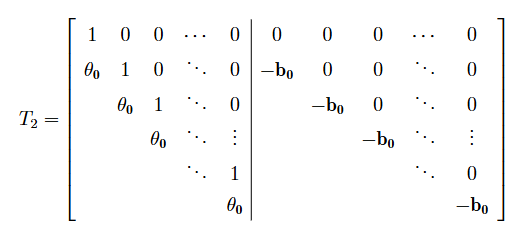
\includegraphics[width=3.08138in,height=1.42003in]{media/image9.png}

\begin{enumerate}
\def\labelenumi{\arabic{enumi}.}
\item
  根据上述维度\(v,m\)以及系统参数\(b_{o}\)构造线性变换\(T_{2}(\theta)\)，并且完成求逆计算，选取合适的控制器，然而只有处理\(v = 2\)系统时才具有关于\(\theta\)的线性滤波性质。
\end{enumerate}

\begin{longtable}[]{@{}
  >{\raggedright\arraybackslash}p{(\linewidth - 2\tabcolsep) * \real{0.0573}}
  >{\raggedright\arraybackslash}p{(\linewidth - 2\tabcolsep) * \real{0.9427}}@{}}
\toprule\noalign{}
\begin{minipage}[b]{\linewidth}\raggedright
\end{minipage} & \begin{minipage}[b]{\linewidth}\raggedright
\[v = 2\]
\end{minipage} \\
\midrule\noalign{}
\endhead
\bottomrule\noalign{}
\endlastfoot
\(m = 1\) &
\(\frac{1}{b_{0}\left( b_{0}^{2} + b_{1}^{2}\theta_{1} \right)}\begin{bmatrix}
 - b_{0}^{2}\theta_{1} & b_{0}b_{1}\theta_{1} & b_{0}^{2} & - b_{0}b_{1} & b_{1}^{2}
\end{bmatrix}\) \\
\(m = 2\) &
\(\frac{1}{b_{0}(b_{0}^{4} + \theta_{1}b_{0}^{2}b_{1}^{2} + \theta_{2}b_{1}^{4})}\begin{bmatrix}
 - b_{0}^{2}(b_{0}^{2}\theta_{1} + b_{1}^{2}\theta_{2}) & b_{0}(b_{0}^{2}b_{1}\theta_{1} - b_{1}^{3}\theta_{2}) & b_{0}^{4} & - b_{0}^{3}b_{1} & b_{0}^{2}b_{1}^{2} & - b_{0}b_{1}^{3} & b_{1}^{4}
\end{bmatrix}\) \\
\(m = 3\) &
\(\frac{1}{b_{0}\left( b_{0}^{6} + \theta_{1}b_{0}^{4}b_{1}^{2} + \theta_{2}b_{0}^{2}b_{1}^{4} + \theta_{3}b_{1}^{6} \right)}\)

\(\begin{bmatrix}
 - b_{0}(\theta_{1}b_{0}^{5} + \theta_{2}b_{0}^{3}b_{1}^{2} + \theta_{3}b_{0}b_{1}^{4}) & b_{0}(\theta_{1}b_{0}^{4}b_{1} + \theta_{2}b_{0}^{2}b_{1}^{3} + \theta_{3}b_{1}^{5}) & b_{0}^{6} & - b_{0}^{5}b_{1} & b_{0}^{4}b_{1}^{2} & - b_{0}^{3}b_{1}^{3} & {b_{0}^{2}b}_{1}^{4} & - b_{0}b_{1}^{5} & b_{1}^{6}
\end{bmatrix}\) \\
\end{longtable}

\begin{longtable}[]{@{}
  >{\raggedright\arraybackslash}p{(\linewidth - 2\tabcolsep) * \real{0.1180}}
  >{\raggedright\arraybackslash}p{(\linewidth - 2\tabcolsep) * \real{0.8820}}@{}}
\toprule\noalign{}
\begin{minipage}[b]{\linewidth}\raggedright
\end{minipage} & \begin{minipage}[b]{\linewidth}\raggedright
\[m = 1\]
\end{minipage} \\
\midrule\noalign{}
\endhead
\bottomrule\noalign{}
\endlastfoot
\(v = 3\) &
\(\frac{1}{b_{0}\left( b_{0}^{2} + \left( b_{1}^{2} - 2b_{2}b_{0} \right)\theta_{1} + b_{2}^{2}\theta_{1}^{2} \right)}\)

\(\begin{bmatrix}
 - b_{0}b_{1}\theta_{1} & b_{0}(b_{2}\theta_{1}^{2} - b_{0}\theta_{1}) & b_{0}b_{1}\theta_{1} & b_{0}({- b}_{2}\theta_{1} + b_{0}) & - b_{0}b_{1} & \left( b_{1}^{2} - b_{2}b_{0} \right) + b_{2}^{2}\theta_{1}
\end{bmatrix}\) \\
\(v = 10\) & \(\begin{aligned}
1/b_{0}\lbrack b_{0}^{2} + & \left( b_{1}^{2} - 2b_{0}b_{2} \right)\theta_{1} + \left( b_{2}^{2} + 2b_{0}b_{4} - 2b_{1}b_{3} \right)\theta_{1}^{2} \\
 + & (b_{3}^{2} - 2b_{0}b_{6} + 2b_{1}b_{5} - \ 2b_{2}b_{4})\theta_{1}^{3} + (b_{4}^{2} + 2b_{0}b_{8} - 2b_{1}b_{7} + 2b_{2}b_{6} - 2b_{3}b_{5})\theta_{1}^{4} \\
 + & \left( b_{5}^{2} + 2b_{1}b_{9} - 2b_{2}b_{8} + \ 2b_{3}b_{7} - 2b_{4}b_{6} \right)\theta_{1}^{5} + \left( b_{6}^{2} - 2b_{3}b_{9} + 2b_{4}b_{8} - 2b_{5}b_{7} \right)\theta_{1}^{6} \\
 + & (b_{7}^{2} + 2b_{5}b_{9} - 2b_{6}b_{8})\theta_{1}^{7} + (b_{8}^{2} - 2b_{7}b_{9})\theta_{1}^{8} + b_{9}^{2}\theta_{1}^{9}\rbrack
\end{aligned}\)

\(\left\lbrack \begin{aligned}
 - b_{0} & \left( b_{8}\theta_{1}^{9} - b_{6}\theta_{1}^{8} + b_{4}\theta_{1}^{7} - b_{2}\theta_{1}^{6} + b_{0}\theta_{1}^{5} \right) \\
b_{0} & \left( b_{8}\theta_{1}^{8} - b_{6}\theta_{1}^{7} + b_{4}\theta_{1}^{6} - b_{2}\theta_{1}^{5} + b_{0}\theta_{1}^{4} \right) \\
 - b_{0} & \left( b_{9}\theta_{1}^{8} - b_{7}\theta_{1}^{7} + b_{5}\theta_{1}^{6} - b_{3}\theta_{1}^{5} + b_{1}\theta_{1}^{4} \right) \\
 - b_{0} & \left( b_{8}\theta_{1}^{7} - b_{6}\theta_{1}^{6} + b_{4}\theta_{1}^{5} - b_{2}\theta_{1}^{4} + b_{0}\theta_{1}^{3} \right) \\
b_{0} & \left( b_{9}\theta_{1}^{7} - b_{7}\theta_{1}^{6} + b_{5}\theta_{1}^{5} - b_{3}\theta_{1}^{4} + b_{1}\theta_{1}^{3} \right) \\
b_{0} & \left( b_{8}\theta_{1}^{6} - b_{6}\theta_{1}^{5} + b_{4}\theta_{1}^{4} - b_{2}\theta_{1}^{3} + b_{0}\theta_{1}^{2} \right) \\
 - b_{0} & \left( b_{9}\theta_{1}^{6} - b_{7}\theta_{1}^{5} + b_{5}\theta_{1}^{4} - b_{3}\theta_{1}^{3} + b_{1}\theta_{1}^{2} \right) \\
 - b_{0} & \left( b_{8}\theta_{1}^{5} - b_{6}\theta_{1}^{4} + b_{4}\theta_{1}^{3} - b_{2}\theta_{1}^{2} + b_{0}\theta_{1} \right) \\
b_{0} & \left( b_{9}\theta_{1}^{5} - b_{7}\theta_{1}^{4} + b_{5}\theta_{1}^{3} - b_{3}\theta_{1}^{2} + b_{1}\theta_{1} \right) \\
b_{0} & \left( b_{8}\theta_{1}^{4} - b_{6}\theta_{1}^{3} + b_{4}\theta_{1}^{2} - b_{2}\theta_{1} + b_{0} \right) \\
 - b_{0} & \left( b_{9}\theta_{1}^{4} - b_{7}\theta_{1}^{3} + b_{5}\theta_{1}^{2} - b_{3}\theta_{1} + b_{1} \right) \\
\begin{aligned}
\left( b_{1}^{2} - \ b_{0}b_{2} \right) + & (b_{2}^{2} + \ b_{0}b_{4} - \ 2\ b_{1}b_{3})\theta_{1} \\
 + & (b_{3}^{2} - \ b_{0}b_{6} + \ 2\ b_{1}b_{5} - \ 2\ b_{2}b_{4})\theta_{1}^{2} \\
 + & (b_{4}^{2} + \ b_{0}b_{8} - \ 2\ b_{1}b_{7} + \ 2\ b_{2}b_{6} - \ 2\ b_{3}b_{5})\theta_{1}^{3} \\
 + & (b_{5}^{2} + \ 2\ b_{1}b_{9} - \ 2\ b_{2}b_{8} + \ 2\ b_{3}b_{7} - \ 2\ b_{4}b_{6})\theta_{1}^{4} \\
 + & \left( b_{6}^{2} - \ 2\ b_{3}b_{9} + \ 2\ b_{4}b_{8} - \ 2\ b_{5}b_{7} \right)\theta_{1}^{5} \\
 + & \left( b_{7}^{2} + \ 2\ b_{5}b_{9} - \ 2\ b_{6}b_{8} \right)\theta_{1}^{6} \\
 + & (b_{8}^{2} - \ 2\ b_{7}b_{9})\theta_{1}^{7} + \ b_{9}^{2}\theta_{1}^{8}
\end{aligned}
\end{aligned} \right\rbrack^{\top}\) \\
\(v = 20\) & ？ \\
\end{longtable}

\begin{enumerate}
\def\labelenumi{\arabic{enumi}.}
\setcounter{enumi}{1}
\item
  选取适当的特征值，构建观测参数\(\lambda\)，系数向量\(d = \left\lbrack 1,d_{2},\ldots,\ d_{v + 2m + 1} \right\rbrack^{\top}\)，构建Hurwitz矩阵\(D\)；
\item
  为每个参数更新选取合适的参数自适应系数\(g_{i},\ i = 1,\ldots,m\)，泄漏因子\(\alpha_{i},\ i = 1,\ldots,m\)。
\item
  根据\(D\)设计大于其时间常数的参数\(\lambda_{0}\)，根据频率下限\(\omega_{\min}\)确定外系统周期的上界\(T_{M}\)，这些参数用于统计\(M_{i}(t)\)，确认是否泄漏。
\end{enumerate}

\subsubsection{仿真验证}\label{ux4effux771fux9a8cux8bc1}

\section{Marino2021理论基础}\label{marino2021ux7406ux8bbaux57faux7840}

\begin{longtable}[]{@{}
  >{\raggedright\arraybackslash}p{(\linewidth - 0\tabcolsep) * \real{1.0000}}@{}}
\toprule\noalign{}
\begin{minipage}[b]{\linewidth}\raggedright
\textbf{线性系统的调节问题如下}：

\[\begin{aligned}
\dot{x} = & Ax + bu + Dz,\ \ x \in \mathbf{R}^{n},u \in \mathbf{R} \\
\dot{z} = & Rz,\ \ z \in \mathbf{R}^{2p + 1} \\
e = & {cx + rz,\ \ y}_{r} = - rz,\ \ y = cx,\ \ y,y_{r},e \in \mathbf{R}
\end{aligned}\]

干扰\(Dz\)和参考输出\(- rz\)均由\textbf{稳定的}线性外系统\(R\)生成。

\textbf{要求}：设计仅由\(e\)驱动的反馈控制器，\(\forall x(0)\)，所有的信号都有界，且随着\(t \rightarrow \infty,\ \ e(t) \rightarrow \infty\)。问题有解的几个充要条件是：

（A1）外系统不稳定（unstable）：不失一般性假设外系统不稳定：\(\mathfrak{R}\left( \lambda(R) \right) \geq 0\)

研究中设\(R\)的特征值为\(0, \pm j\omega_{1},\ldots, \pm j\omega_{p}\)，均在虚轴上。

（A2）可稳性（stabilizable）：\((A,b)\)可稳：\(\mathfrak{R}(\lambda) < 0,\ \ rank\begin{bmatrix}
\lambda I - A & b
\end{bmatrix} < n\)；

（A3）可检测性（detectable）：\((A,c)\)可测：\(\mathfrak{R}(\lambda) < 0,\ \ rank\begin{bmatrix}
\lambda I - A \\
c
\end{bmatrix} < n\)

（A4）传输零点条件（Transmission zero
Condtion）：\(\forall\lambda(R),rank\left( \begin{bmatrix}
\lambda(R)I - A & b \\
c & 0
\end{bmatrix} \right) = n + 1\)，即此矩阵行满秩。换言之，\(R\)的特征值与系统传函的传输零点不重合。

\textbf{以上Assumption共同构成了线性输出调节问题有解的条件。}
\end{minipage} \\
\midrule\noalign{}
\endhead
\bottomrule\noalign{}
\endlastfoot
\end{longtable}

注意输出调节问题有解的上述假设并不强制要求被控对象\(P(s)\)为最小相位的（既不要求所有极点在LHP，也不要求零点在LHP）。在上述条件下，调节问题可转化为\textbf{增广系统}的误差反馈镇定问题，其中状态误差向量
ξ 与误差 e(t) 均应被驱至零，以使 u 产生偏置多正弦信号 γz。

\begin{longtable}[]{@{}
  >{\raggedright\arraybackslash}p{(\linewidth - 0\tabcolsep) * \real{1.0000}}@{}}
\toprule\noalign{}
\begin{minipage}[b]{\linewidth}\raggedright
\textbf{增广系统的输出反馈镇定问题}

令\(\xi = \lbrack x,\ z\rbrack\)

\[\begin{aligned}
\dot{\xi} = & A\xi + b(u - \gamma z),\ \ x \in \mathbf{R}^{n},u \in \mathbf{R} \\
\dot{z} = & Rz,\ \ z \in \mathbf{R}^{2p + 1} \\
e = & {c\xi,\ \ y}_{r} = - rz,\ \ y = cx,\ \ y,y_{r},e \in \mathbf{R}
\end{aligned}\]
\end{minipage} \\
\midrule\noalign{}
\endhead
\bottomrule\noalign{}
\endlastfoot
\end{longtable}

自2003年以来，Marino等学者一直致力于寻找调节问题有界的最简先验条件。其中一个基本问题是，\textbf{为了设计基于误差反馈的调节器，对具有相对阶}\(\rho\)\textbf{和高频增益}\(k_{p}\)\textbf{的传递函数，需要多少先验知识？}

2015年，Marino等人在研究中指出，只要知道\(P(0)\)及\(\mathfrak{R}\left( P(j\omega_{i}) \right)\)的符号，即可为稳定且可观测的不确定线性系统设计低增益误差反馈调节器。

2021年，Marino等人将研究拓展至最小相位系统的高增益调节器。\textbf{高增益调节器在控制系统设计中具有独特的优势，尤其适用于处理不确定性和扰动抑制问题。例如，在面对系统的不确定性或外部扰动时，高增益可以增强系统对这些不确定性或扰动的抑制能力。对于可能不稳定的最小相位系统，设计高增益调节器可以利用其高增益特性来克服系统的不稳定因素，提高系统的稳定性和性能。这使得研究这类系统的高增益调节器设计具有重要的理论和实际意义。}

研究旨在回答，对于最小相位的SISO线性系统，设计输出反馈调节器的最少先验信息是什么。研究给出的答案是：只需要高频增益\(k_{p}\)的符号和相对阶的上界\(\overline{\rho}\)，即可设计一个阶次为\(\overline{\rho} + 2p\)的高增益、实有理（proper）、稳定的调节器（其中\(p\)为外系统阶次）。在外系统特征值完全已知的条件下，该调节器仅依赖单个可调参数\(k\)。

\subsection{完整的控制器结构}\label{ux5b8cux6574ux7684ux63a7ux5236ux5668ux7ed3ux6784-1}

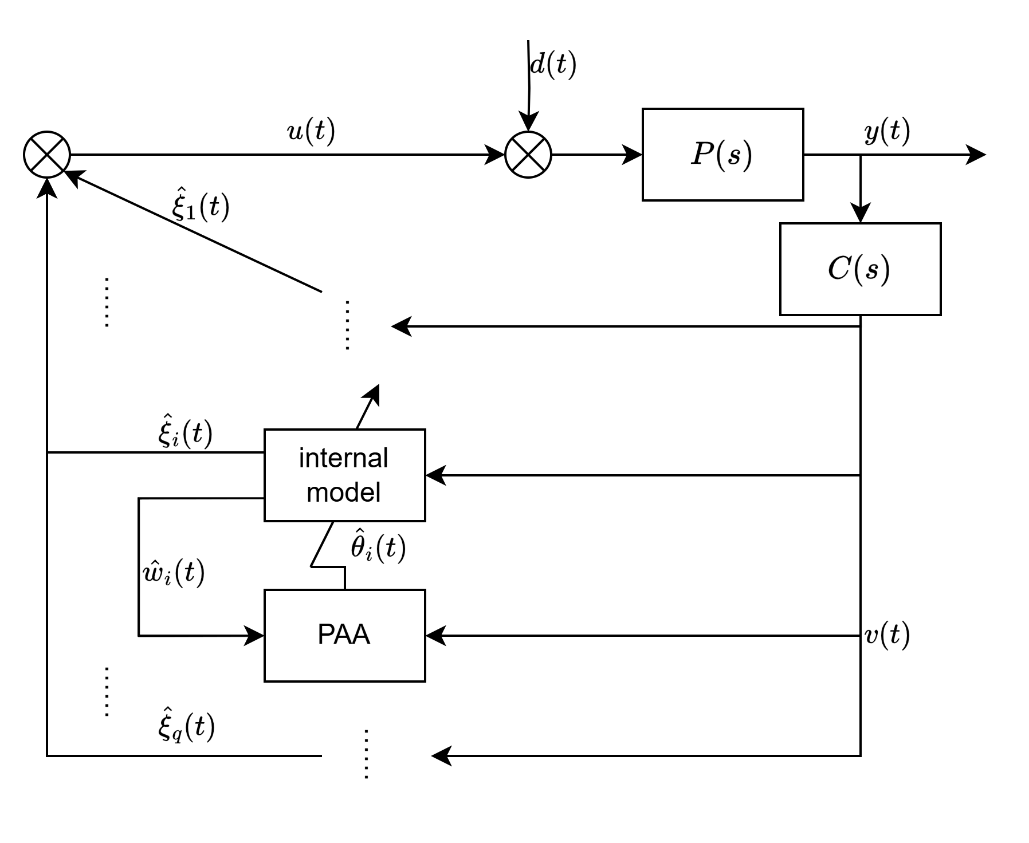
\includegraphics[width=4.67639in,height=3.83264in]{media/image10.png}

控制器明显由两部分组成：

\textbf{高增益线性补偿}\(v(s) = - C(s)y(s)\)和\textbf{自适应内模/并联自适应滤波器组}\(u(s) = \sum_{i = 0}^{q}{\widehat{\xi}}_{i}\)

\subsection{已知外系统}\label{ux5df2ux77e5ux5916ux7cfbux7edf}

\subsection{不确定外系统}\label{ux4e0dux786eux5b9aux5916ux7cfbux7edf}

\section{附录：最小相位系统}\label{ux9644ux5f55ux6700ux5c0fux76f8ux4f4dux7cfbux7edf}

文章研究的被控对象仅限于能观的最小相位系统。

这一假设对于regulator equation可解至关重要。

\begin{itemize}
\item
  \textbf{稳定性与可控性}
  ：最小相位系统的所有极点和零点都在复平面的左半部分，这意味着系统是稳定的，并且可以通过反馈控制来调节其动态行为。在设计调节器时，可以利用这一特性来确保闭环系统的稳定性。
\item
  \textbf{适应性} ：在（Marino, Tomei,
  2007）中提到的直接自适应方法中，最小相位假设允许设计一个相对简单的控制算法，该算法可以在不知道外系统确切参数的情况下，通过在线估计和调整来实现对系统的调节。这提高了控制策略的适应性和灵活性。
\item
  \textbf{鲁棒性}
  ：最小相位系统对参数的不确定性和外部扰动具有更好的鲁棒性。这使得在设计调节器时，可以更好地处理系统中的未知因素和扰动，如（Marino,
  Tomei, 2007）中提到的未知频率的正弦信号。
\item
  \textbf{收敛性} ：（Marino, Tomei,
  2007）中提到，如果所有外系统的频率都被激发，那么在最小相位假设下，调节误差会指数收敛到零。这种快速的收敛性对于实际应用中的控制系统是非常重要的，意味着系统可以更快地达到期望的运行状态。
\end{itemize}

\section{附录：能稳性、能观性}\label{ux9644ux5f55ux80fdux7a33ux6027ux80fdux89c2ux6027}

\section{附录：Lyapunov函数在稳定性分析中的作用}\label{ux9644ux5f55lyapunovux51fdux6570ux5728ux7a33ux5b9aux6027ux5206ux6790ux4e2dux7684ux4f5cux7528}

\section{附录：能观标准型、最小实现、状态观测器}\label{ux9644ux5f55ux80fdux89c2ux6807ux51c6ux578bux6700ux5c0fux5b9eux73b0ux72b6ux6001ux89c2ux6d4bux5668}

\section{附录：控制器的离散化问题}\label{ux9644ux5f55ux63a7ux5236ux5668ux7684ux79bbux6563ux5316ux95eeux9898}

我们知道，使用数字控制器控制连续系统的方法有两种：（1）先对连续系统设计一个连续控制器，再将其离散化为一个离散控制器；（2）先将连续系统离散化为离散系统，再针对它设计一个离散控制器。\textbf{在控制理论遵循前一种设计思路，多从连续域模型出发}；在ANC领域所接触到的控制器则大多直接将对象建模为离散系统，再使用数字信号处理的相关理论设计离散域的滤波器。

自动化专业的学生在本科课程当中更加熟悉的是连续域的控制理论，对于离散域模型知之甚少或不够熟悉，课程教学中也常常有意回避这一部分，似乎是在刻意与通信学科划清界限。当然我们没有必要特别去强调两种设计思路的差异。但是需要认识到要实现从连续控制器到它的滤波器实现，中间是需要一定的理论基础作为过渡的。这一过渡的理论就是控制器离散化问题。

对连续时间积分进行数值近似存在两种做法。一是将连续时间的微分方程模型近似为离散时间的差分方程模型，这种近似采取的方法是数值积分方法；二是将连续时间的传递函数模型近似为离散时间的传递函数模型，这种技术采取的方法是多种变换。事实上这两种做法存在一定的对应关系，这一知识点在自动控制原理B课程中得到一定的讲解。

\begin{longtable}[]{@{}
  >{\centering\arraybackslash}p{(\linewidth - 2\tabcolsep) * \real{0.5000}}
  >{\centering\arraybackslash}p{(\linewidth - 2\tabcolsep) * \real{0.5000}}@{}}
\toprule\noalign{}
\begin{minipage}[b]{\linewidth}\centering
\textbf{变换方法/替换法}
\end{minipage} & \begin{minipage}[b]{\linewidth}\centering
\textbf{数值积分近似方法}
\end{minipage} \\
\midrule\noalign{}
\endhead
\bottomrule\noalign{}
\endlastfoot
Z变换/冲激响应不变 & \\
带有虚拟ZOH的Z变换 & \\
一阶差分近似（前向差分/后向差分） & 欧拉法 \\
双线性变换/预畸变的双线性变换 & 梯形积分 \\
根匹配法 & \\
& 龙格-库塔法 \\
\end{longtable}

\subsection{数值积分方法：微分方程→差分方程}\label{ux6570ux503cux79efux5206ux65b9ux6cd5ux5faeux5206ux65b9ux7a0bux5deeux5206ux65b9ux7a0b}

微分方程组数值求解，将微分方程转换为差分方程。哈深为研究生开设一门数值分析课程。大概简介一下课程内容。

\subsubsection{前向欧拉法（Forward
Euler）}\label{ux524dux5411ux6b27ux62c9ux6cd5forward-euler}

\subsubsection{后向欧拉法（Backward
Euler）}\label{ux540eux5411ux6b27ux62c9ux6cd5backward-euler}

\subsubsection{梯形法（Trapezoidal）}\label{ux68afux5f62ux6cd5trapezoidal}

\subsubsection{龙格-库塔法（Runge-Kutta）}\label{ux9f99ux683c-ux5e93ux5854ux6cd5runge-kutta}

\subsection{连续系统离散化：连续传函→离散传函}\label{ux8fdeux7eedux7cfbux7edfux79bbux6563ux5316ux8fdeux7eedux4f20ux51fdux79bbux6563ux4f20ux51fd}

在YouTube上的控制领域博主Brian
Douglas对MATLAB提供的控制器离散化方法作了讲解。

\subsubsection{Impulse冲激响应不变法}\label{impulseux51b2ux6fc0ux54cdux5e94ux4e0dux53d8ux6cd5}

\subsubsection{ZOH零阶保持/阶跃响应不变法}\label{zohux96f6ux9636ux4fddux6301ux9636ux8dc3ux54cdux5e94ux4e0dux53d8ux6cd5}

\subsubsection{FOH
线性插值/一阶保持/斜坡响应不变法}\label{foh-ux7ebfux6027ux63d2ux503cux4e00ux9636ux4fddux6301ux659cux5761ux54cdux5e94ux4e0dux53d8ux6cd5}

\subsubsection{Matched
零极点匹配法}\label{matched-ux96f6ux6781ux70b9ux5339ux914dux6cd5}

\subsubsection{Tustin
双线性变换及预畸变处理}\label{tustin-ux53ccux7ebfux6027ux53d8ux6362ux53caux9884ux7578ux53d8ux5904ux7406}

\subsection{经典ANC算法的连续时间模型}\label{ux7ecfux5178ancux7b97ux6cd5ux7684ux8fdeux7eedux65f6ux95f4ux6a21ux578b}

\section{附录：模型参考自适应控制}\label{ux9644ux5f55ux6a21ux578bux53c2ux8003ux81eaux9002ux5e94ux63a7ux5236}

阅读文章的过程中，经由sgn(P)已知这一假设，使我联想到了非线性与自适应控制这门课程中所讲过的模型参考自适应控制（MRAC）/自适应控制设计。在这部分理论中也使用了关于系统的这一信息。不知道是否有对\textbf{符号假设}的说明（控制理论中为什么会引入这种假设？如何直观理解符号假设的重要性所在？）。

\section{附录：自适应反馈线性化与滤波变换}\label{ux9644ux5f55ux81eaux9002ux5e94ux53cdux9988ux7ebfux6027ux5316ux4e0eux6ee4ux6ce2ux53d8ux6362}

\subsection{（1）Marino Tomei变换}\label{marino-tomeiux53d8ux6362}

考虑单输入不确定（uncertain）系统

\(\dot{x} = f(x) + q\left( x,\theta(t) \right) + g(x)u \triangleq \overline{f}\left( x,\theta(t) \right) + g(x)u,\ \ x \in \mathbf{R}^{n},u \in \mathbf{R},\ \theta \in \Omega \subset \mathbf{R}^{p}\)，

其中\(f,g\)为已知的光滑向量场，其中存在一个不受\(\theta(t)\)影响的孤立平衡点

\[f(0) = 0,\ \ q(0,\theta) = 0,\ \ \forall\theta \in \Omega\]

函数\(q(x,\theta) = \overline{f}(x,\theta) - \overline{f}(x,\overline{\theta})\)，关于\(x,\theta\)光滑且包含所有可能的不确定性；

\(\theta(t)\)为紧子集\(\Omega\)内未知时变且分段连续的干扰向量，定义标称常向量\(\overline{\theta}\)（\(\overline{f}\left( x,\overline{\theta} \right) = f(x)\)）。

书中第2章对于无干扰、且参数和非线性精确已知的系统提供了一些反馈线性化方法。而第3章需要处理的问题则是不确定系统的状态反馈控制设计。文中提供了能够保证控制存在的几类不确定系统，并试图给出构造性的设计步骤。包括如下：

\begin{enumerate}
\def\labelenumi{\arabic{enumi}.}
\item
  \textbf{三角型结构}
\item
  \textbf{鲁棒镇定}：干扰和不确定性参数（有界）以非线性的形式加入系统；
\item
  \textbf{自校正调节器}：干扰和不确定性参数（有界）以线性形式加入系统；
\item
  \textbf{自适应控制（MRAC/AFL）}：常值未知参数。
\end{enumerate}

所有这些自适应技术都是为了克服\textbf{标准反馈线性化}对\textbf{模型精确性}的依赖，扩展其在存在不确定性和干扰时的适用性。

\subsection{（2）1983 Isidori
输出注入和非线性观测的线性}\label{isidori-ux8f93ux51faux6ce8ux5165ux548cux975eux7ebfux6027ux89c2ux6d4bux7684ux7ebfux6027}

\subsubsection{（2.1）观测器和输出注入}\label{ux89c2ux6d4bux5668ux548cux8f93ux51faux6ce8ux5165}

\paragraph{问题制定}\label{ux95eeux9898ux5236ux5b9a}

\subsubsection{（2.2）基于非线性输出注入的线性化}\label{ux57faux4e8eux975eux7ebfux6027ux8f93ux51faux6ce8ux5165ux7684ux7ebfux6027ux5316}

文章给出了两条路线。若\(L_{f}(dh)\)线性依赖于低阶项，则只通过坐标变换即可实现线性化（命题1、命题2表述）；若进一步满足李括号条件，可以同时做坐标变换和非线性输出注入。

\paragraph{能观性假设（Observability
Assumption）}\label{ux80fdux89c2ux6027ux5047ux8bbeobservability-assumption}

定义非线性系统：

\[\begin{aligned}
\dot{x} = & \mathbf{f}(x) \\
y = & h(x)
\end{aligned}\]

若系统在感兴趣点\(x^{0}\)的某邻域\(U\)上\(x \in U\)有：\(L_{f}^{k}(dh)(x),k = 0,\ldots,n - 1\)线性独立，则系统能观。

其中一阶微分\(\mathbf{d}h = \mathbf{\nabla}h(x)^{\top} = \left( \frac{\partial h(x)}{\partial x_{1}},\ \ldots,\ \frac{\partial h(x)}{\partial x_{n}} \right)\)是\textbf{输出动态}的梯度，此梯度对\textbf{状态向量场}\(f\)的李导数\(L_{f}(\mathbf{d}h)\)，\textbf{行梯度定义（numerator
layout）}。

\[L_{f}h(x) = \mathbf{d}h(x)\mathbf{f}(x) = \mathbf{\nabla}h(x)^{\top}\mathbf{f}(x) = \left( \frac{\partial h(x)}{\partial x_{1}},\ \ldots,\ \frac{\partial h(x)}{\partial x_{n}} \right)\mathbf{f}(x) = \sum_{j = 1}^{n}{\frac{\partial h(x)}{\partial x_{j}}f_{j}(x)}\]

\[\begin{aligned}
\mathbf{d}\left( L_{f}h \right)(x) = & \mathbf{\nabla}\left( \mathbf{\nabla}h^{\top}\mathbf{f} \right)^{\top} = \mathbf{f}^{\top}\nabla^{2}h + \nabla h^{\top}\nabla\mathbf{f} \\
 = & \left( \frac{\partial L_{f}h(x)}{\partial x_{1}},\ \ldots,\ \frac{\partial L_{f}h(x)}{\partial x_{n}} \right) \\
 = & \left( \sum_{j = 1}^{n}\left( \frac{\partial^{2}h(x)}{\partial x_{1}\partial x_{j}}f_{j}(x) + \frac{\partial h(x)}{\partial x_{j}}\frac{\partial f_{j}(x)}{\partial x_{1}} \right),\ldots,\sum_{j = 1}^{n}\left( \frac{\partial^{2}h(x)}{\partial x_{n}\partial x_{j}}f_{j}(x) + \frac{\partial h(x)}{\partial x_{j}}\frac{\partial f_{j}(x)}{\partial x_{n}} \right) \right) \\
 = & \mathbf{f}(x)\frac{\partial^{2}h(x)}{\partial x^{2}} + \left( \frac{\partial h(x)}{\partial x_{1}},\ \ldots,\ \frac{\partial h(x)}{\partial x_{n}} \right)\frac{\partial\mathbf{f}(x)}{\partial x} \\
 = & L_{f}\left( \mathbf{d}h \right)(x)
\end{aligned}\]

对于线性系统

\[\begin{aligned}
\dot{x} = & Ax \\
y = & Cx
\end{aligned},\ \ \mathbf{d}h = \nabla h^{\top} = C,\ \ J_{f} = \nabla\mathbf{f} = A\]

\[\begin{aligned}
L_{f}\left( \mathbf{d}h \right)(x) = & \mathbf{f}^{\top}\nabla^{2}h + \nabla h^{\top}\nabla\mathbf{f} = 0 + CA \\
L_{f}^{2}\left( \mathbf{d}h \right)(x) = & \left( \nabla h^{\top}\nabla\mathbf{f} \right)\nabla\mathbf{f =}CA^{2} \\
L_{f}^{k}\left( \mathbf{d}h \right)(x) = & CA^{k}
\end{aligned}\]

\paragraph{命题1
坐标线性化的充要条件}\label{ux547dux98981-ux5750ux6807ux7ebfux6027ux5316ux7684ux5145ux8981ux6761ux4ef6}

\[\left\{ \begin{array}{r}
\dot{x} = f(x) \\
y = h(x)
\end{array} \right.\  \leftarrow \xi = \xi(x) \rightarrow \left\{ \begin{array}{r}
\dot{\xi} = A\xi \\
y = C\xi
\end{array} \right.\ \]

坐标变换\(\xi = \xi(x),\ \ \xi\left( x^{0} \right) = 0\)使得\textbf{非线性系统}与上述\textbf{线性系统}局部等价，

当且仅当\(f\left( x^{0} \right) = 0,h\left( x^{0} \right) = 0\)且\(L_{f}^{n}\left( \mathbf{d}h \right) = CA^{n}\)可写作\(L_{f}^{k}\left( \mathbf{d}h \right) = CA^{k},\ k = 0,\ \ldots,n - 1\)的线性组合。

\paragraph{命题2
坐标线性化条件的李括号表述}\label{ux547dux98982-ux5750ux6807ux7ebfux6027ux5316ux6761ux4ef6ux7684ux674eux62ecux53f7ux8868ux8ff0}

\[\left\{ \begin{array}{r}
\dot{x} = f(x) \\
y = h(x)
\end{array} \right.\  \leftarrow \xi = \xi(x) \rightarrow \left\{ \begin{array}{r}
\dot{\xi} = A\xi \\
y = C\xi
\end{array} \right.\ \]

坐标变换\(\xi = \xi(x),\ \ \xi\left( x^{0} \right) = 0\)使得\textbf{非线性系统}与上述\textbf{线性系统}局部等价，

当且仅当\(f\left( x^{0} \right) = 0,h\left( x^{0} \right) = 0\)且存在如下定义的向量场\(g(x)\)

\(L_{g}L_{f}^{n}(h) = \left\{ \begin{aligned}
0, & 0 \leq k < n - 1 \\
1, & k = n - 1
\end{aligned} \right.\ \)，\(\left\lbrack g,{ad}^{k}(f)g \right\rbrack = 0,\ \ k = 1,3,\ldots,2n - 1\)。

若存在这样的坐标变换，也可以将变换为\textbf{能观伴随型（observable
companion form）线性系统}。

\[\begin{aligned}
\mathbf{f}(x) = & Ax = \begin{bmatrix}
a_{1} & 1 & \ldots & 0 \\
 \vdots & & \ddots & \\
a_{n - 1} & 0 & & 1 \\
a_{n} & 0 & \ldots & 0
\end{bmatrix}\begin{bmatrix}
x_{1} \\
 \vdots \\
x_{n}
\end{bmatrix} \\
y = & Cx = \begin{bmatrix}
1 & 0 & \ldots & 0
\end{bmatrix}\begin{bmatrix}
x_{1} \\
 \vdots \\
x_{n}
\end{bmatrix}
\end{aligned}\]

当系统已经写成能观伴随型后，只需用\(G\)把输出\(y\)注入到状态方程中\(u = Gy\)，就能在不破坏结构的前提下，任意改变系统的第一列（即最左侧那一列系数）；这正是\textbf{线性输出注入}在\textbf{能观标准型}里的简洁体现。\(\dot{x} = Ax + u = (A + GC)x\)

\paragraph{命题3
含非线性输出注入的线性化条件}\label{ux547dux98983-ux542bux975eux7ebfux6027ux8f93ux51faux6ce8ux5165ux7684ux7ebfux6027ux5316ux6761ux4ef6}

\[\left\{ \begin{array}{r}
\dot{x} = f(x) \\
y = h(x)
\end{array} \right.\  \leftarrow \xi = \xi(x) \rightarrow \left\{ \begin{aligned}
\dot{\xi} = & A\xi + \varphi(y) \\
y = & C\xi
\end{aligned} \right.\ \]

坐标变换\(\xi = \xi(x),\ \ \xi\left( x^{0} \right) = 0\)使得\textbf{非线性系统}与上述\textbf{含非线性输出注入的线性系统}局部等价，

当且仅当\(f\left( x^{0} \right) = 0,h\left( x^{0} \right) = 0\)且存在如下定义的向量场\(g(x)\)

\(L_{g}L_{f}^{n}(h) = \left\{ \begin{aligned}
0, & 0 \leq k < n - 1 \\
1, & k = n - 1
\end{aligned} \right.\ \)，\(\left\lbrack g,{ad}^{k}(f)g \right\rbrack = 0,\ \ k = 1,3,\ldots,2n - 3\)。

\section{附录：反馈逆控制}\label{ux9644ux5f55ux53cdux9988ux9006ux63a7ux5236}

\subsection{前馈开环高增益控制}\label{ux524dux9988ux5f00ux73afux9ad8ux589eux76caux63a7ux5236}

\href{https://www.zhihu.com/question/448429887}{(39 封私信 / 11 条消息)
控制理论中到底什么是high gain control？ - 知乎}

本质上，所有控制器均在可行范围内隐式生成对象逆。控制器的差异在于生成所需近似逆的机制不同。实际对象模型往往无法精确求逆。但反馈具有\textbf{隐含生成动态变换近似逆}的特性，无需显式执行反演。其中一种结构涉及到将被控对象逆替换为以下结构，其中\(h\)待定：

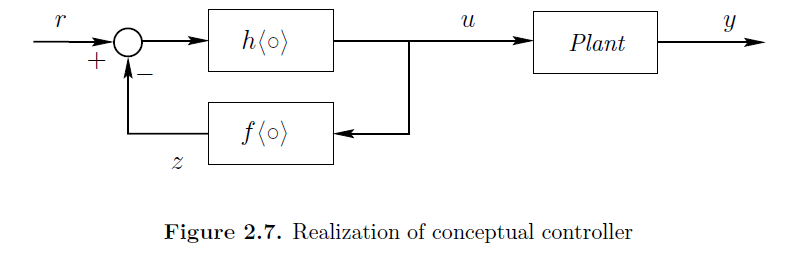
\includegraphics[width=4.2045in,height=1.3237in]{media/image11.png}

\[u = h\left\langle r - f(u) \right\rangle = f^{- 1}\left\langle r - h^{- 1}\left\langle u \right\rangle \right\rangle\]

因此，环路在\(r \approx r - h^{- 1}\left\langle u \right\rangle\)时能够近似被控对象的逆\(f^{- 1}\)，而这一条件在\(h\)具有高增益时得到满足。换言之，当\(h^{- 1}\)可忽略（即\(h\)为\textbf{高增益变换}）时系统隐式构造近似逆。

需要注意的是，这种控制器以开环方式作用于对象。核心问题在于：控制信号\(u(t)\)与被控对象的实际状态完全解耦，这种架构仅当满足以下严苛条件时才可行：

\begin{enumerate}
\def\labelenumi{\arabic{enumi}.}
\item
  模型精度：控制器设计所基于的模型需要高度匹配实际对象；
\item
  稳定性约束：模型及其逆变换均需是稳定的（BIBO且最小相位的？）；
\item
  扰动抑制：外部干扰与初始条件的影响可忽略。
\end{enumerate}

\textbf{此外，高环路增益通过近似逆实现控制本质，但实际工程中选择反馈增益需融入复杂的设计权衡网络。理解并平衡这些权衡，正是控制系统设计的精髓所在。}

\begin{enumerate}
\def\labelenumi{\arabic{enumi}.}
\item
  \textbf{执行器饱和约束}：若\(e(t)\)不为0，则高增益反馈生成的控制作用\(u(t)\)极大，可能超出执行器的可用输入范围，使解决方案失效；
\item
  \textbf{严重的稳定性问题}：失稳特性表现为自持振荡（甚至增幅振荡）。典型示例是当扬声器距离麦克风过近时产生的高频啸叫声------这正是过度反馈增益引发的失稳现象。悲剧性的失稳案例包括多起空难事故，以及因失控状态导致的切尔诺贝利核灾难。
\item
  \textbf{对测量噪声的敏感性}：
\end{enumerate}

\subsection{反馈闭环控制架构}\label{ux53cdux9988ux95edux73afux63a7ux5236ux67b6ux6784}

为解决前馈控制结构的必然缺陷，需改进方案以\textbf{保留核心思想}同时\textbf{引入对象本身的反馈}：

\begin{enumerate}
\def\labelenumi{\arabic{enumi}.}
\item
  \textbf{基础结构}：基于图2.9的基本反馈架构进行重构；
\item
  \textbf{理想假设下}：若模型完美匹配对象，可推导出图2.10的替代方案；
\item
  \textbf{本质转变}：该方案将反馈回路从模型迁移至实际对象，形成闭环控制的基础。
\end{enumerate}

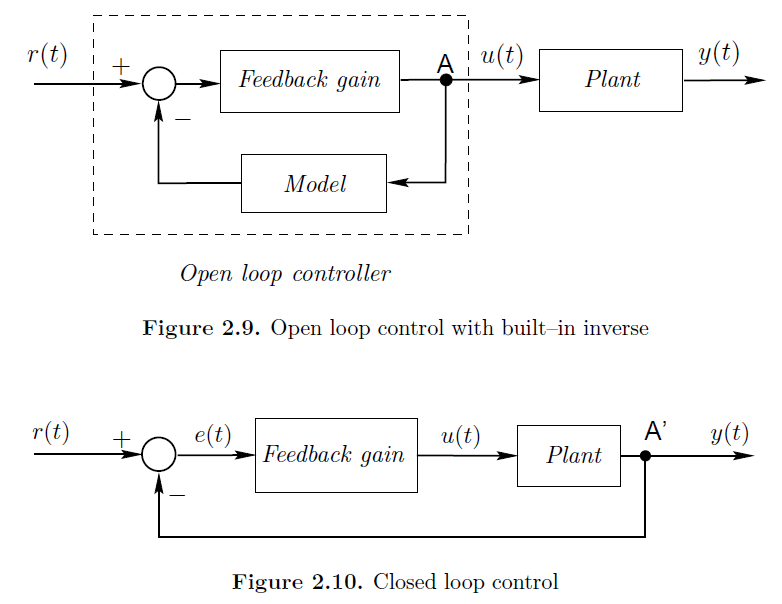
\includegraphics[width=3.28324in,height=2.53611in]{media/image12.png}

\begin{enumerate}
\def\labelenumi{\arabic{enumi}.}
\item
  \textbf{等效性条件}：当模型完全匹配对象且所有信号有界（回路稳定）时，两架构在~\emph{r}(\emph{t})~到~\emph{y}(\emph{t})~的传递关系上等价。
\item
  \textbf{本质差异}：闭环架构通过\textbf{实时测量过程变量}，从根本上提升对扰动和初始条件的鲁棒性。
\end{enumerate}

\begin{longtable}[]{@{}
  >{\raggedright\arraybackslash}p{(\linewidth - 4\tabcolsep) * \real{0.1749}}
  >{\raggedright\arraybackslash}p{(\linewidth - 4\tabcolsep) * \real{0.4144}}
  >{\raggedright\arraybackslash}p{(\linewidth - 4\tabcolsep) * \real{0.4107}}@{}}
\toprule\noalign{}
\begin{minipage}[b]{\linewidth}\raggedright
\textbf{对比维度}
\end{minipage} & \begin{minipage}[b]{\linewidth}\raggedright
\textbf{开环架构（图2.9）}
\end{minipage} & \begin{minipage}[b]{\linewidth}\raggedright
\textbf{闭环架构（图2.10）}
\end{minipage} \\
\midrule\noalign{}
\endhead
\bottomrule\noalign{}
\endlastfoot
\textbf{反馈信号来源} & 控制器内部点A（计算机/硬件内部） &
对象实际输出A\textquotesingle（通过传感器测量） \\
\textbf{抗扰能力} & 依赖模型精度，抗扰弱 & 实时修正扰动影响 \\
\textbf{工程实现} & 纯计算实现 & 需部署外部测量设备 \\
\end{longtable}

\section{参考文献}\label{ux53c2ux8003ux6587ux732e}

\begin{enumerate}
\def\labelenumi{\arabic{enumi}.}
\item
  GOODWIN G C, GRAEBE S F, SALGADO M E. Control System Design{[}M{]}.
  Upper Saddle River: Prentice Hall, 2001.
\item
  MARINO R, SANTOSUOSSO G L, TOMEI P. Robust adaptive compensation of
  biased sinusoidal disturbances with unknown frequency{[}J/OL{]}.
  Automatica, 2003, 39(10): 1755-1761.
  DOI:\href{https://doi.org/10.1016/S0005-1098(03)00170-5}{10.1016/S0005-1098(03)00170-5}.
\item
  MARINO R, TOMEI P. Output regulation for linear systems via adaptive
  internal model{[}J/OL{]}. IEEE Transactions on Automatic Control,
  2003, 48(12): 2199-2202.
  DOI:\href{https://doi.org/10.1109/TAC.2003.820143}{10.1109/TAC.2003.820143}.
\item
  MARINO R, SANTOSUOSSO G L. On the linear regulator with unknown stable
  exosystems{[}C/OL{]}//2004 43rd IEEE Conference on Decision and
  Control (CDC) (IEEE Cat. No.04CH37601): 卷 5. 2004: 4571-4576
  Vol.5{[}2025-02-28{]}.
  \url{https://ieeexplore.ieee.org/document/1429504}.
  DOI:\href{https://doi.org/10.1109/CDC.2004.1429504}{10.1109/CDC.2004.1429504}.
\item
  MARINO R, TOMEI P. Adaptive Regulation of Uncertain Linear Minimum
  Phase Systems with Unknown Exosystems{[}C/OL{]}//Proceedings of the
  45th IEEE Conference on Decision and Control. 2006:
  1099-1104{[}2025-03-02{]}.
  \url{https://ieeexplore.ieee.org/document/4177216}.
  DOI:\href{https://doi.org/10.1109/CDC.2006.377667}{10.1109/CDC.2006.377667}.
\item
  MARINO R, SANTOSUOSSO G L. Regulation of Linear Systems With Unknown
  Exosystems of Uncertain Order{[}J/OL{]}. IEEE Transactions on
  Automatic Control, 2007, 52(2): 352-359.
  DOI:\href{https://doi.org/10.1109/TAC.2006.890376}{10.1109/TAC.2006.890376}.
\item
  MARINO R, TOMEI P. Output Regulation for Linear Minimum Phase Systems
  With Unknown Order Exosystem{[}J/OL{]}. IEEE Transactions on Automatic
  Control, 2007, 52(10): 2000-2005.
  DOI:\href{https://doi.org/10.1109/TAC.2007.904288}{10.1109/TAC.2007.904288}.
\item
  MARINO R, TOMEI P. Adaptive Regulator for Uncertain Linear Minimum
  Phase Systems with Unknown Undermodeled Exosystems{[}J/OL{]}. IFAC
  Proceedings Volumes, 2008, 41(2): 11293-11298.
  DOI:\href{https://doi.org/10.3182/20080706-5-KR-1001.01913}{10.3182/20080706-5-KR-1001.01913}.
\item
  MARINO R, TOMEI P. An adaptive learning regulator for uncertain
  minimum phase systems with undermodeled unknown exosystems{[}J/OL{]}.
  Automatica, 2011, 47(4): 739-747.
  DOI:\href{https://doi.org/10.1016/j.automatica.2011.01.019}{10.1016/j.automatica.2011.01.019}.
\item
  BASTURK H I, KRSTIC M. Adaptive wave cancelation by acceleration
  feedback for ramp-connected air cushion-actuated surface effect
  ships{[}J/OL{]}. Automatica, 2013, 49(9): 2591-2602.
  DOI:\href{https://doi.org/10.1016/j.automatica.2013.05.017}{10.1016/j.automatica.2013.05.017}.
\item
  MARINO R, TOMEI P. Disturbance cancellation for linear systems by
  adaptive internal models{[}J/OL{]}. Automatica, 2013, 49(5):
  1494-1500.
  DOI:\href{https://doi.org/10.1016/j.automatica.2013.02.011}{10.1016/j.automatica.2013.02.011}.
\item
  MARINO R, TOMEI P. Global Adaptive Regulation of Uncertain Nonlinear
  Systems in Output Feedback Form{[}J/OL{]}. IEEE Transactions on
  Automatic Control, 2013, 58(11): 2904-2909.
  DOI:\href{https://doi.org/10.1109/TAC.2013.2258794}{10.1109/TAC.2013.2258794}.
\item
  MARINO R, TOMEI P. Output Regulation for Unknown Stable Linear
  Systems{[}J/OL{]}. IEEE Transactions on Automatic Control, 2015,
  60(8): 2213-2218.
  DOI:\href{https://doi.org/10.1109/TAC.2014.2368234}{10.1109/TAC.2014.2368234}.
\item
  MARINO R, TOMEI P. Adaptive disturbance rejection for unknown stable
  linear systems{[}J/OL{]}. Transactions of the Institute of Measurement
  and Control, 2016, 38(6): 640-647.
  DOI:\href{https://doi.org/10.1177/0142331215625769}{10.1177/0142331215625769}.
\item
  MARINO R, TOMEI P. Hybrid Adaptive Multi-Sinusoidal Disturbance
  Cancellation{[}J/OL{]}. IEEE Transactions on Automatic Control, 2017,
  62(8): 4023-4030.
  DOI:\href{https://doi.org/10.1109/TAC.2016.2615978}{10.1109/TAC.2016.2615978}.
\item
  MARINO R, TOMEI P. Adaptive output regulation for minimum-phase
  systems with unknown relative degree{[}J/OL{]}. Automatica, 2021, 130:
  109670.
  DOI:\href{https://doi.org/10.1016/j.automatica.2021.109670}{10.1016/j.automatica.2021.109670}.
\item
  TOMEI P, MARINO R. Adaptive regulation for minimum phase systems with
  unknown relative degree and uncertain exosystems{[}J/OL{]}.
  Automatica, 2023, 147: 110678.
  DOI:\href{https://doi.org/10.1016/j.automatica.2022.110678}{10.1016/j.automatica.2022.110678}.
\item
  A generalized projection estimation algorithm{[}J/OL{]}. Automatica,
  2025, 171: 111942.
  DOI:\href{https://doi.org/10.1016/j.automatica.2024.111942}{10.1016/j.automatica.2024.111942}.
\end{enumerate}

\end{document}
